% JNCA manuscript based on Elsevier's officially recommended elsarticle class.
% The scientific text is carried over from the previously revised English manuscript.
\documentclass[preprint,12pt,authoryear]{elsarticle}
\journal{Journal of Network and Computer Applications}
\usepackage{amsmath,amssymb,amsthm,booktabs,graphicx,tabularx}
\usepackage{url}
\emergencystretch=2em
\newtheorem{proposition}{Proposition}
\newtheorem{lemma}{Lemma}
\begin{document}
\begin{frontmatter}
\title{Zero-Knowledge Certification of Robust Spacetime Compliance under Byzantine Evidence for Vehicular Crowdsensing}
\author[univ]{Lili He}
\author[univ]{Sheng Jiang}
\author[univ]{Shuang Chen}
\author[univ]{Lei Zhang\corref{cor1}}
\cortext[cor1]{Corresponding author.}
\ead{8213662@163.com}
\address[univ]{College of Information and Electronic Technology, Jiamusi University, Jiamusi 154007, China}
\begin{abstract}
In vehicular crowdsensing, a location-privacy mechanism may need to establish compliance with a spatial policy without revealing a vehicle's coordinates. Yet positioning errors, environmental effects, and synchronization uncertainty often leave only interval-valued spacetime observations. Even authenticated sources may share systematic bias or behave in a Byzantine manner. We propose a privacy-preserving compliance certification method based on signed spacetime uncertainty evidence. Given an upper bound $f$ on Byzantine issuers and an allowance $r$ for honest issuers whose intervals miss the true event, the method constructs the feasible set of states supported by at least $k=n-f-r$ issuers. A report is accepted only when this set is nonempty and wholly contained in the authorized region. The resulting decision distinguishes valid, invalid, ambiguous, and inconsistent evidence. We implement two Groth16/BN254 circuits that verify EdDSA/MiMC signatures and bind the proof to the task, issuer roster, report, threshold, challenge nonce, and expiry. Gateway tests reject tampering, context substitution, expired challenges, and cross-challenge replay; only one of eight concurrent copies of a valid request is accepted within a single gateway instance. Across 12 synthetic conditions satisfying the configured fault and coverage assumptions, mean decisive coverage is 87.52\%, compared with 75.63\% for a fixed-margin baseline. Tested subset circuits produce 164-byte proofs with median proving times of 163--255 ms on an Apple M1. The implementation is an evidence-certification layer, not a complete vehicular crowdsensing platform; its physical interpretation still depends on trusted issuer enrollment and effective sensor calibration.
\end{abstract}
\begin{keyword}
Zero-knowledge proofs \sep Location privacy \sep Vehicular crowdsensing \sep Byzantine evidence \sep Robust evidence fusion \sep Spacetime compliance certification
\end{keyword}
\end{frontmatter}
\section{Introduction}
In location-privacy applications, a verifier may need to establish that a user satisfies a spatial policy without learning the user's precise coordinates. Zero-knowledge location proofs, for example, can verify membership in a designated region while keeping the location private ~\citep{ZKLP,VehiclePolicy}. Such verification commonly starts from a definite spacetime position. Vehicle sensing, however, cannot always provide an observation of that kind. Positioning error, environmental interference, and clock-synchronization uncertainty may restrict the available evidence to a range of plausible positions and times. A valid source signature authenticates the evidence submitted by that source; it does not establish that the physical estimate is accurate. Compromised sources may also sign deliberately misleading observations. Consequently, even a mathematically correct proof concerning a hidden coordinate does not establish that the chosen coordinate is sufficiently supported by observations. This paper asks how multiple uncertain, and potentially malicious, spacetime observations can support a policy-compliance claim without being disclosed to the verifier.

The problem is particularly relevant to vehicular crowdsensing. Distributed vehicle observations support traffic monitoring, road management, and environmental-sensing tasks ~\citep{Suhag2023,Zheng2025BARM}, for which the admissibility of a report may depend on the event's location and time. Revealing the positioning evidence can expose a vehicle's mobility history. Replacing several interval-valued observations with one representative point, however, can conceal disagreement near a policy boundary. Requiring every source interval to intersect is not necessarily safer: a Byzantine issuer may submit a displaced interval that excludes the true state while leaving a small intersection entirely within the authorized region. A sound compliance rule therefore needs to specify which possible states have sufficient evidential support and how conflicting observations are handled, in addition to protecting those observations.

We consider privacy-preserving compliance certification over signed spacetime uncertainty evidence. Each enrolled issuer signs an axis-aligned integer box for the same reference event. For $n$ issuers, at most $f$ Byzantine sources, and at most $r$ honest observations that fail to cover the true state, let $k = n - f - r$. The robust feasible set $\mathcal{F}_k$ consists of the states covered by at least $k$ signed boxes. Compliance is certified only if this set is nonempty and entirely contained in the authorized policy. A nonempty feasible set lying outside the policy produces an invalid decision; a set crossing the boundary is ambiguous; and a set with no threshold-supported state is inconsistent. A valid decision is reserved for the acceptance condition. These four outcomes avoid treating an arbitrarily chosen point as conclusive and distinguish a conflict in otherwise valid evidence from failure to submit the required evidence.

The support-depth construction builds on classical fault-tolerant interval fusion, including the threshold-intersection principle of Marzullo; our contribution is its exact zero-knowledge certification, circuit construction, and report-bound gateway enforcement.

We combine threshold-based fault-tolerant interval reasoning ~\citep{Marzullo1990,BFTPoLoc,PG,CRSF} with zero-knowledge certification. Rather than revealing the source intervals, the prover establishes that the signatures satisfy the roster and context constraints and that the reported decision follows from the same threshold rule. A report-binding protocol associates this proof with the task, issuer roster, report bytes, threshold, challenge nonce, and expiry. This association prevents a proof for one authorized context from being reused as evidence for another, under the stated cryptographic and gateway assumptions.

In a conventional gateway-side fusion design, submitting each signed uncertainty box to the verifier would reveal sensitive spatiotemporal positioning envelopes and make them available for retention or cross-task linkage. Our setting instead permits the gateway to learn the task context, report and final classification, but not the source boxes or their signed private witness. This asymmetry motivates an exact zero-knowledge certificate rather than merely running the threshold rule on disclosed evidence.

Designed as a modular evidence-certification component for vehicular crowdsensing architectures, our framework focuses on source authentication, contextual binding, and verifiable set-level compliance, while treating participant recruitment, incentive mechanisms, and physical sensor calibration as orthogonal upstream services. We explicitly separate these physical coverage premises from cryptographic guarantees throughout the security analysis.

The contributions are summarized as follows:
\begin{itemize}
\item \textbf{Four-valued certification under explicit fault and coverage budgets.} We use the set of threshold-supported spacetime states as the object of policy verification, distinguish valid, invalid, ambiguous, and inconsistent evidence, and establish conditional soundness when the true state is covered by sufficiently many honest sources.
\item \textbf{Two exact finite-domain proof circuits.} Lower-corner maximum-depth reachability and threshold-subset enumeration establish the same four-valued relation. Both are instantiated with Groth16/BN254, verify EdDSA/MiMC signatures within the circuit, and constrain the private evidence to the public policy, roster, threshold, and report context.
\item \textbf{A task-bound verification gateway.} The gateway reconstructs public inputs from a trusted task configuration, checks roster consistency, verifies the proof, and atomically marks a successfully used challenge as consumed. Protocol tests examine evidence tampering, task/report substitution, expired challenges, and concurrent replay within one gateway instance.
\item \textbf{Comprehensive semantic and cryptographic evaluation.} We evaluate the framework across 64,800 synthetic observations, paired ablations over honest-miscoverage allowances, trajectory replay on 787 measured UrbanNav reference states with simulated multisource evidence, 300 Groth16 proof executions across both circuit backends, resource-limited R1CS compilation sweeps, and a same-runner comparison against an open-source location-proof baseline.
\end{itemize}

Figure~\ref{fig:architecture} depicts the certificate workflow. Issuers authenticate uncertainty regions associated with the same report; the vehicle uses the regions and signatures as a private witness; and the gateway checks the public task context and accepts the report only after verifying a valid classification. The witness is hidden from the verifier, while the report content, public policy, and classification remain visible.

\begin{figure}[htbp]\centering
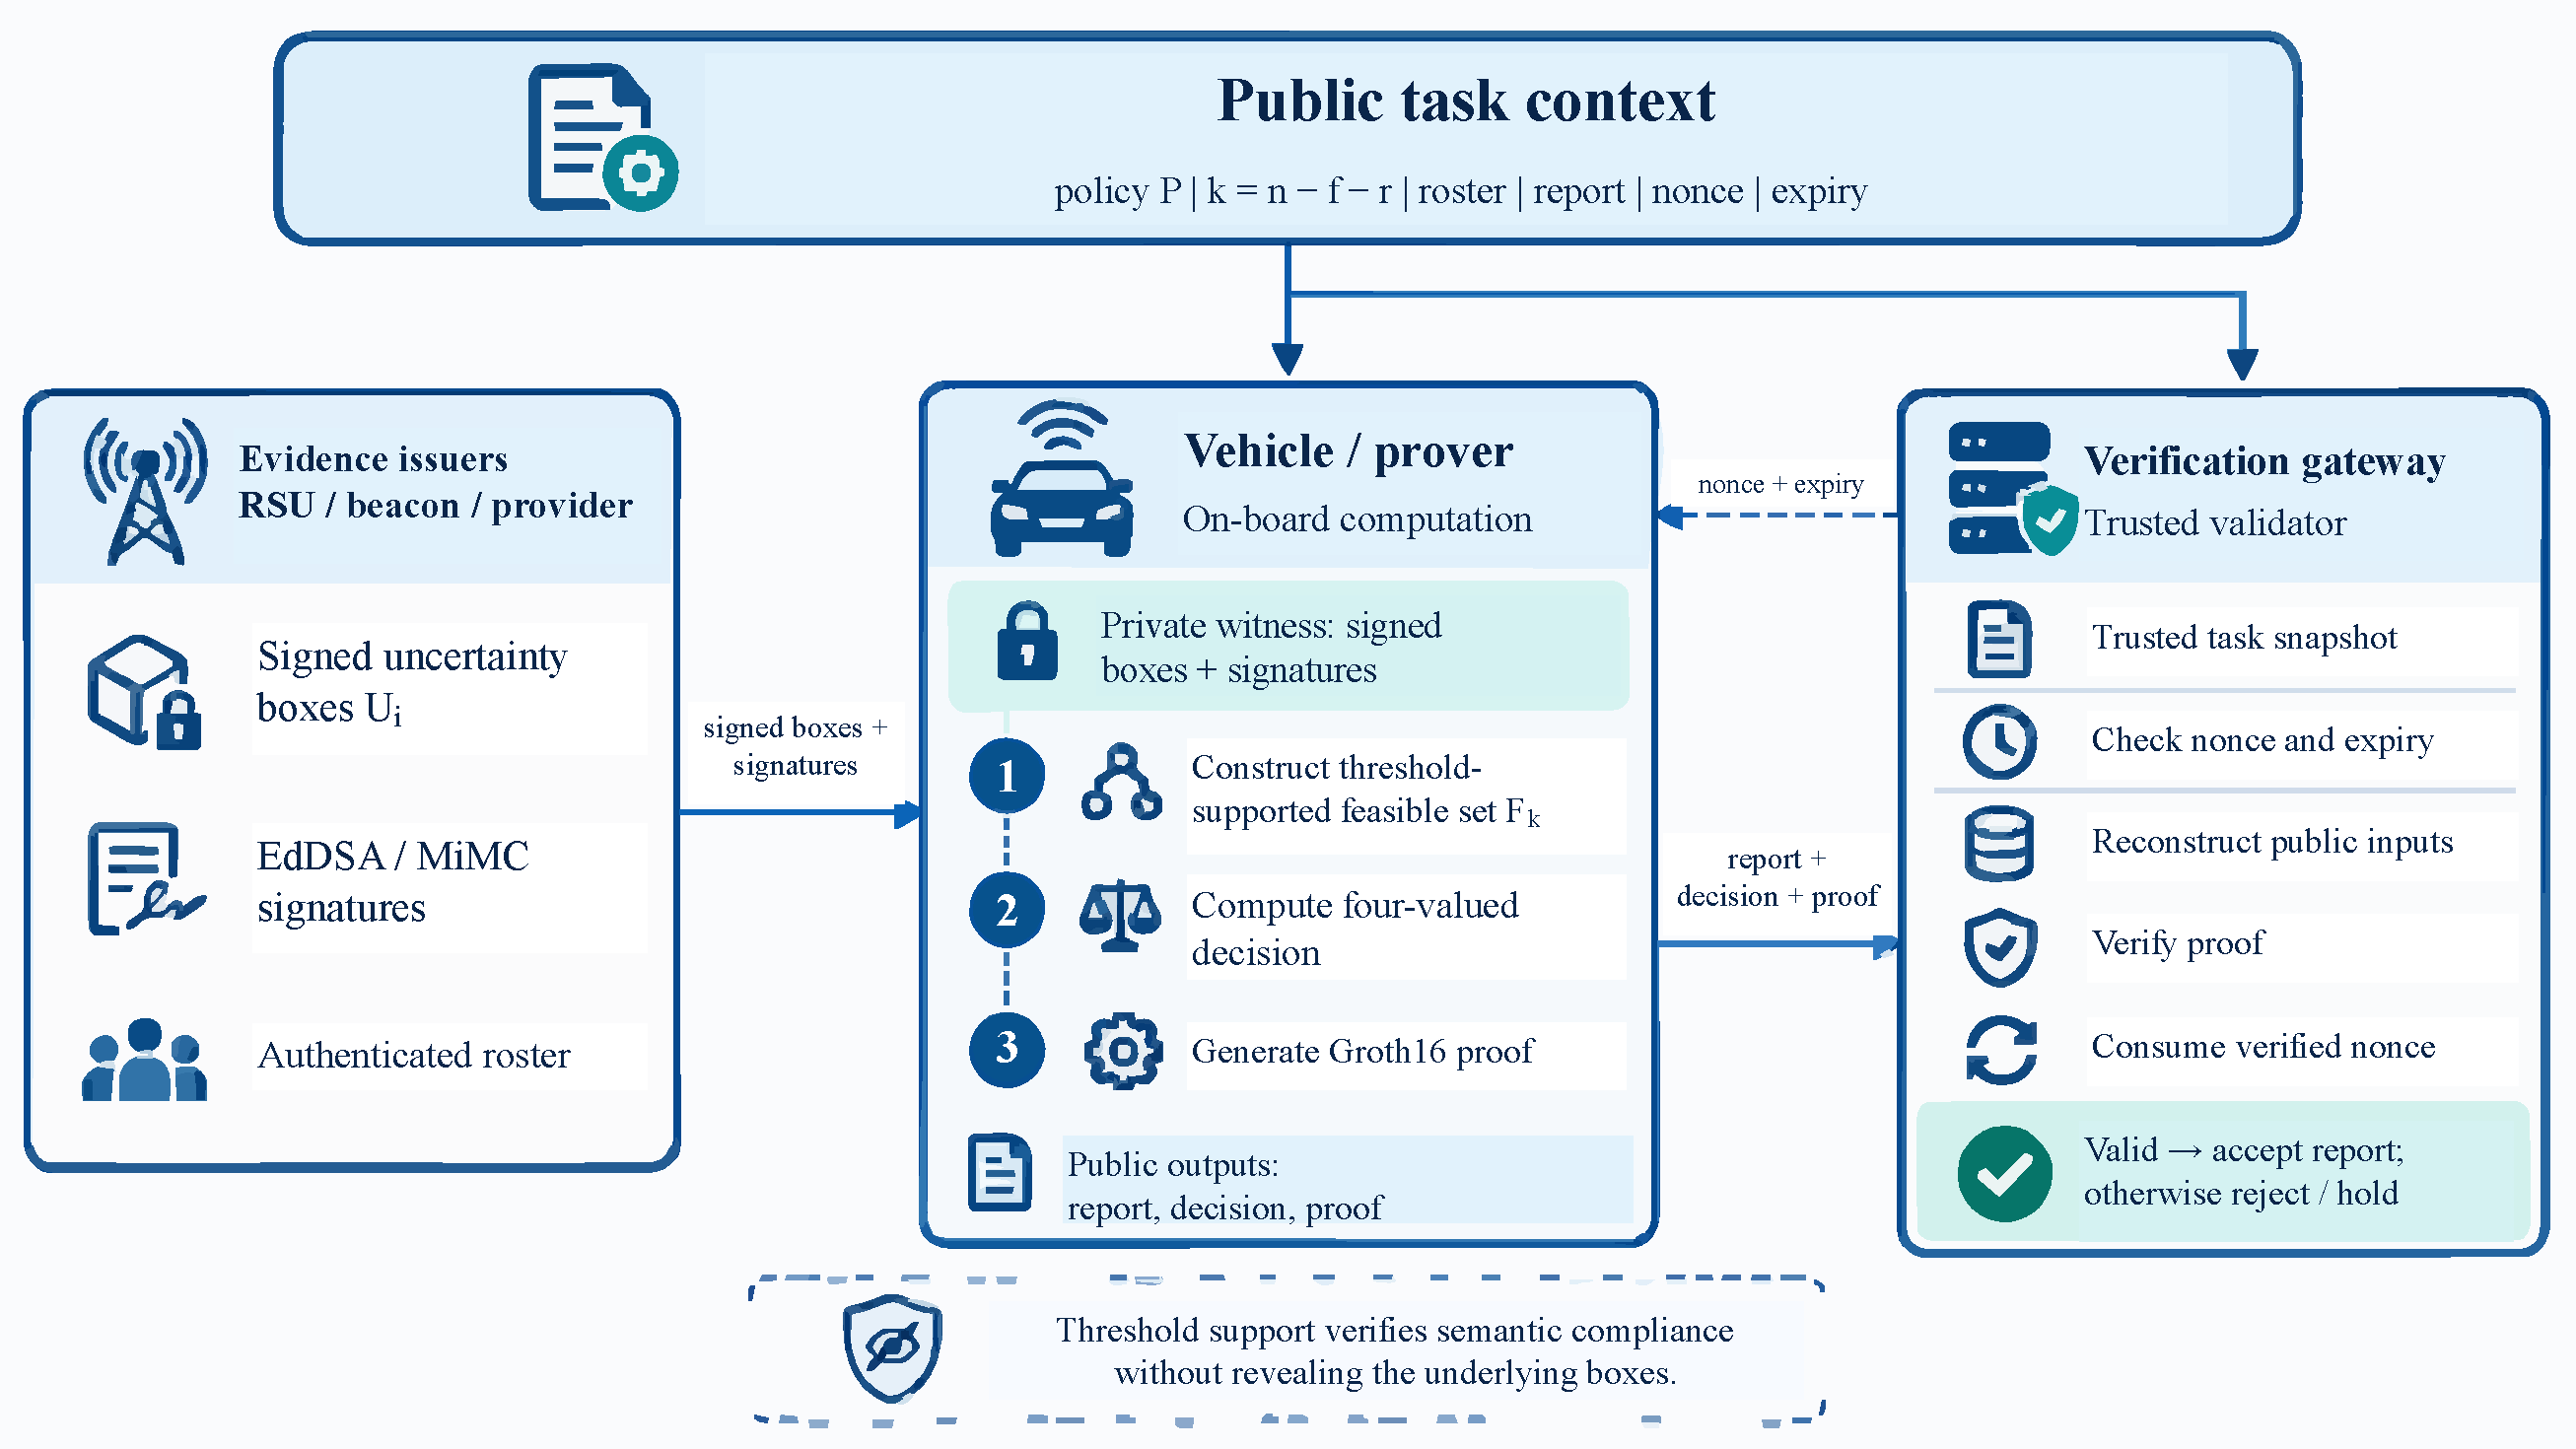
\includegraphics[width=\linewidth]{system_architecture.pdf}
\caption{Conceptual architecture of the evidence-certification module. Signed boxes $U_i$ contribute to the threshold-supported feasible set $\mathcal{F}_k$ in a quantized integer domain. An inconsistent decision represents a semantic outcome over complete, authenticated evidence, whereas missing or malformed evidence aborts the protocol. This schematic was generated with AI assistance (OpenAI ChatGPT).}\label{fig:architecture}
\end{figure}

Section 2 reviews relevant work on vehicular privacy, zero-knowledge location verification, and Byzantine-robust fusion. Section 3 develops the model and circuits; Section 4 establishes their security boundary; Section 5 presents the experiments; Section 6 discusses deployment and interoperability, and Section 7 concludes.
\section{Related Work}
\subsection{Privacy and trustworthy crowdsensing in vehicular networks}
Research on vehicular crowdsensing security has addressed participant identity, confidentiality of sensed data, and evidence trustworthiness. AARE combines anonymous authentication with privacy-preserving assessment of data reliability~\citep{Cheng2023}. BARM introduces blockchain-assisted anonymous authentication and reputation management to evaluate and update participant reputations~\citep{Zheng2025BARM}. Regarding data processing, PPVDA studies privacy-preserving and verifiable aggregation~\citep{Zhou2024}; BCS-LPP employs techniques including Geohash and order-preserving encryption to protect sensing locations while supporting location checks and task management~\citep{Shen2024}. Cooperative detection of anomalous vehicular behavior has also been investigated at both vehicle and roadside-unit levels~\citep{Sultana2024}. Other recent work examines lightweight anonymous authentication, certificateless aggregate signatures, and SNARK-based verification of computations on authenticated data~\citep{Imam2025JISA,Wang2025JISA,Reinhart2026ADSC}. Recent VANET work in the \emph{Journal of Network and Computer Applications} also studies conditional privacy-preserving message authentication with secret-key updates~\citep{JNCaFan2026}; its authentication objective is distinct from proving the spatial compliance of mutually uncertain signed reports.

At the vehicular edge, Li et al. study fog-based IoV security using post-quantum signcryption and blockchain-supported trust management~\citep{JNCaLi2025}. Their work addresses secure communications and dynamic trust, while our module concentrates on the semantics of authenticated spacetime uncertainty.

Authentication has also been studied in other adversarial network settings. Umrani and Palmieri examine threshold password-authenticated key exchange for vehicular ad hoc networks~\citep{CybersecUmrani2025}, while Wang et al. develop multi-authority aggregate signatures for privacy-preserving message authentication in smart grids~\citep{CybersecWang2026}. Their security objectives concern key establishment and message authenticity, not whether signed measurement regions physically cover a reported event.

In mobile crowdsensing, the BLIND system protects data sources and improves truth discovery through encrypted clustering and private outlier handling~\citep{JNCaAgate2024}. It addresses data-quality inference rather than a report-bound certificate that all sufficiently supported spacetime states meet a public policy.

These mechanisms address different parts of the sensing workflow: authentication governs participation, aggregation protects inputs, and misbehavior detection identifies suspicious participants. None of these functions by itself resolves whether an event complies with a policy when authenticated sources provide uncertain or conflicting observations. That decision also needs to account for uncertainty in the individual observations.

\subsection{Zero-knowledge location and geometric-policy verification}
Location privacy can be pursued through application-specific obfuscation and protected queries~\citep{Mdee2022,Atmaca2024}, or by credentials and authentication protocols that limit the disclosure of sensitive location information~\citep{Ghani2025,Zhang2025Sybil,Wang2025ZKAuth}. Zero-knowledge proofs offer another approach: a verifier can check a geometric constraint without learning the protected coordinate or an entire trajectory. ZKLP, proposed by Ernstberger and colleagues, incorporates floating-point geometry into zero-knowledge proofs for region membership and proximity predicates~\citep{ZKLP}. The vehicle-policy protocols of Bogdanov and colleagues instead use locations signed by a trusted witness to prove compliance with driving-area requirements in subsidy or taxation applications~\citep{VehiclePolicy}.

Privacy-preserving policy enforcement has also been examined outside geometric verification. Kerl et al. investigate private attribute-based access decisions using homomorphic encryption and zero-knowledge proofs~\citep{CybersecKerl2025}, while Zhang develops zero-knowledge policy checks over encrypted network traffic~\citep{CybersecZhang2026}. These studies certify attribute or traffic-policy relations rather than threshold support across signed, uncertain spacetime observations.

The location-proof systems discussed above demonstrate that geometric predicates and vehicle-trajectory policies can be certified while withholding the underlying positions. Protecting a position, however, differs from establishing that the asserted position is adequately supported by observations. With disagreeing measurement intervals or sources that may maliciously sign data, proving membership of one chosen point or an existing trajectory does not establish that \emph{all} states supported by sufficient evidence satisfy the policy. Our proof relation therefore concerns the threshold support induced jointly by multiple signed intervals, rather than repeated membership testing of a selected coordinate.

\subsection{Byzantine-robust sensor fusion}
Uncertainty and disagreement across measurements have long been studied in fault-tolerant sensor fusion. Marzullo's approach to continuous-valued sensor failures uses overlapping intervals to characterize states consistent with potentially faulty observations~\citep{Marzullo1990}. BFT-PoLoc applies Byzantine-resistant geometry to localization from Internet delays~\citep{BFTPoLoc}. PG combines private computation and Byzantine-tolerant sensor fusion while addressing output delivery~\citep{PG}. CRSF further examines private fusion when sensors and servers may collude, including participation consistency and protocol liveness~\citep{CRSF}.

These systems handle inconsistent observations and malicious participants; some also provide participation or delivery guarantees beyond those of a fixed issuer roster. Their output is a fused estimate or a secure computation result. Our setting instead calls for a report-bound proof that a verifier can check against a spacetime policy without seeing the signed intervals.

\subsection{Comparison and research positioning}
Table~\ref{tab:related-work} compares the objects verified by these methods, their trust assumptions, and their outputs. Our construction uses threshold support to retain the uncertainty in signed evidence, then proves the resulting set-level policy decision in zero knowledge.

\begin{table}[htbp]\centering\footnotesize
\caption{Functional scope and trust assumptions of representative systems.}\label{tab:related-work}
\begin{tabularx}{\linewidth}{@{}p{0.18\linewidth}p{0.21\linewidth}p{0.29\linewidth}X@{}}
\toprule Method & Object & Evidence and trust assumptions & Privacy and output\\\midrule
BARM~\citep{Zheng2025BARM} & Identity and reputation & Reputation evaluation and blockchain-assisted identity management & Anonymous authentication and private reputation evaluation\\
PPVDA~\citep{Zhou2024} & Sensing aggregates & Homomorphic message authentication, secret sharing, malicious participants & Private inputs and verifiable aggregation\\
BCS-LPP~\citep{Shen2024} & Sensing location & Geohash, order-preserving encryption, deposit mechanism & Location privacy and task/location checking\\
BFT-PoLoc~\citep{BFTPoLoc} & Delay-based location & Internet delays and Byzantine-resistant geometry & Ranging and multilateration; privacy not rated here\\
PG~\citep{PG} & Fused sensor result & Malicious sensors and aggregating servers & Private inputs/results; output-delivery guarantee\\
CRSF~\citep{CRSF} & Fusion and participation & Sensor--server collusion and consistency of submissions & Private fusion, explicit abort and liveness\\
ZKLP~\citep{ZKLP} & Region and proximity & Hidden coordinates; floating-point geometry & Zero-knowledge geometric proof\\
Vehicle policy~\citep{VehiclePolicy} & Driving-area policy & Locations signed by a trusted witness & Hidden trajectory; subsidy and tax compliance\\
\textbf{This work} & \textbf{All threshold-supported spacetime states} & \textbf{Signed uncertainty boxes, fixed roster, budgets $f$ and $r$} & \textbf{Hidden boxes/signatures; report-bound four-valued proof}\\\bottomrule
\end{tabularx}
\par\smallskip\raggedright\footnotesize BFT-PoLoc and CRSF refer to the cited arXiv versions. All privacy and correctness claims depend on their respective trust assumptions. Semantic inconsistency must not be confused with abort on missing evidence or proof failure.
\end{table}

The circuit checks issuer signatures and set-level compliance for a pre-established roster. It produces a compact, noninteractive certificate bound to the task, report, and challenge; the physical interpretation remains conditional on the fault and coverage budgets.

\section{Proposed Framework}
We design a report-bound zero-knowledge compliance method for multisource spacetime observations subject to measurement uncertainty and Byzantine failures. Instead of first collapsing these observations into a single estimated location, the method retains their intervals and evaluates compliance against every possible state reaching a support threshold. The workflow constructs a robust feasible set from signed evidence, determines its relationship to the authorized policy, and proves the resulting decision. We first establish the system model and decision semantics, and then describe the binding protocol and proof circuits.

\subsection{System model and assumptions}
For a reference event associated with a sensing report, write the true spacetime state as $z^* = (x, y, t)$. We represent space and time in a $d$-dimensional discrete domain,


\begin{equation}\label{eq:domain}
\Omega = \left(\prod_{a=1}^{d} [L_a, H_a]\right) \cap \mathbb{Z}^d.
\end{equation}


The interval $[L_a, H_a]$ bounds coordinate $a$. An authorized spacetime policy is a public integer box $P \subseteq \Omega$. Each enrolled evidence issuer $i$ (e.g., an independent roadside unit (RSU), cellular base station, or local positioning beacon) signs an inclusive axis-aligned integer box $U_i \subseteq \Omega$ concerning the same reference event, under a common context $c$. All sources use a common coordinate reference system, time base, measurement units, and conservative quantization rule, where continuous uncertainty regions are mapped to all intersecting integer cells. In the prototype, interval endpoints are encoded as unsigned 16-bit integers, and out-of-range coordinates are rejected prior to circuit execution.

The system comprises evidence issuers, a vehicle acting as prover, and a verification gateway. The host crowdsensing application supplies the authorized task, raw report bytes, fixed roster of $n$ issuers, and calibration settings. The vehicle collects the signed evidence for a report and produces a zero-knowledge proof of its four-valued classification. The gateway verifies the proof under its trusted task configuration and returns a decision.

We assume that among the $n$ enrolled issuers, at most $f$ are Byzantine and may submit arbitrary signed intervals. Up to $r$ further intervals from honest issuers may fail to cover the true state $z^*$, allowing for potentially correlated measurement errors. The gateway enforces roster distinctness by rejecting repeated public keys and trust-domain labels, while organizational independence and Sybil-resistant enrollment are enforced at the registration layer. All $n$ roster members must provide valid signatures for a task; missing or invalid signatures cause the protocol to abort rather than yielding a certified inconsistent decision, making the module suited for delay-tolerant task certification.

Let $l_{ia}$ and $u_{ia}$ be the lower and upper endpoints of $U_i$ in coordinate $a$. The signed message digest is

\begin{equation}\label{eq:signedbox}
m_i = \mathrm{MiMC}(c, i, l_{i1}, u_{i1}, \dots, l_{id}, u_{id}).
\end{equation}


The circuit verifies an EdDSA signature on this digest. Its public statement includes $c$, $\Omega$, $P$, the support threshold $k$, the decision code, and the ordered issuer public keys. The shared context $c$ binds the task, coordinate conventions, policy, threshold, issuer roster, report digest, challenge nonce, and expiry, which the gateway reconstructs directly from its trusted configuration. While cryptographic verification guarantees source authenticity and set-level computation over the quantized domain $\Omega$, inferring physical compliance of $z^*$ relies on the upstream premise that at least $k$ honest uncertainty envelopes physically cover the event.

\subsection{Four-valued robust spacetime compliance}
For uncertain evidence from several sources, membership of one selected point in the authorized region does not suffice to certify the event. We instead impose a set-level requirement: compliance is accepted only if every threshold-supported possible state belongs to the policy and at least one such state exists. Unlike an intersection of all source intervals, this rule allows anomalous intervals to be excluded from the support of an individual state.

For $1\leq k=n-f-r\leq n$, the robust feasible set is
\begin{equation}\label{eq:feasible}
\mathcal F_k=\left\{z\in\Omega:\sum_{i=1}^n\mathbf 1[z\in U_i]\geq k\right\}.
\end{equation}
Here $\mathbf 1[\cdot]$ is the indicator function. Define reachability inside and outside the policy by
\[
I=\mathbf 1[\mathcal F_k\cap P\ne\varnothing],\qquad
O=\mathbf 1[\mathcal F_k\cap(\Omega\setminus P)\ne\varnothing].
\]
The pair $(I,O)$ defines the four mutually exclusive outcomes in Table~\ref{tab:decisions}. Only a Valid classification can authorize acceptance following successful proof verification.

\begin{table}[htbp]\centering\small
\caption{Four-valued robust spacetime compliance.}\label{tab:decisions}
\begin{tabularx}{\linewidth}{@{}ccclX@{}}\toprule
$I$ & $O$ & $\delta$ & Outcome & Feasible-set condition\\\midrule
1&0&0&Valid&$\mathcal F_k\ne\varnothing$ and $\mathcal F_k\subseteq P$\\
0&1&1&Invalid&$\mathcal F_k\ne\varnothing$ and $\mathcal F_k\cap P=\varnothing$\\
1&1&2&Ambiguous&Supported states occur inside and outside $P$\\
0&0&3&Inconsistent&$\mathcal F_k=\varnothing$\\\bottomrule
\end{tabularx}
\end{table}

Inconsistent evidence is a semantic decision computed from a complete set of authenticated signatures. It is not a label for missing signatures, an invalid proof, or an expired nonce. Explicit nonemptiness matters because $\varnothing\subseteq P$ is mathematically true, although an empty feasible set supports no actual event. Conversely, a nonempty feasible set need not contain the physical true state without further assumptions; Section~4 supplies the requisite conditional-soundness argument.

Figure~\ref{fig:counterexample} illustrates how the full-source intersection can disagree with threshold support. Consider $\Omega=[-4,8]\cap\mathbb Z$, $P=[0,8]\cap\mathbb Z$, $n=3$, $f=1$, $r=0$, and $k=2$. Both honest intervals contain the true but noncompliant state $z^\star=-1$. A Byzantine interval excludes this point while leaving the intersection of all three intervals equal to $[2,4]\cap\mathbb Z$. Accepting on that intersection could therefore be incorrect. The threshold-supported set is instead $[-2,4]\cap\mathbb Z$ and spans the policy boundary, correctly producing an Ambiguous decision. This is a constructed illustration of the semantics, not an experimental observation.
\begin{figure}[htbp]\centering
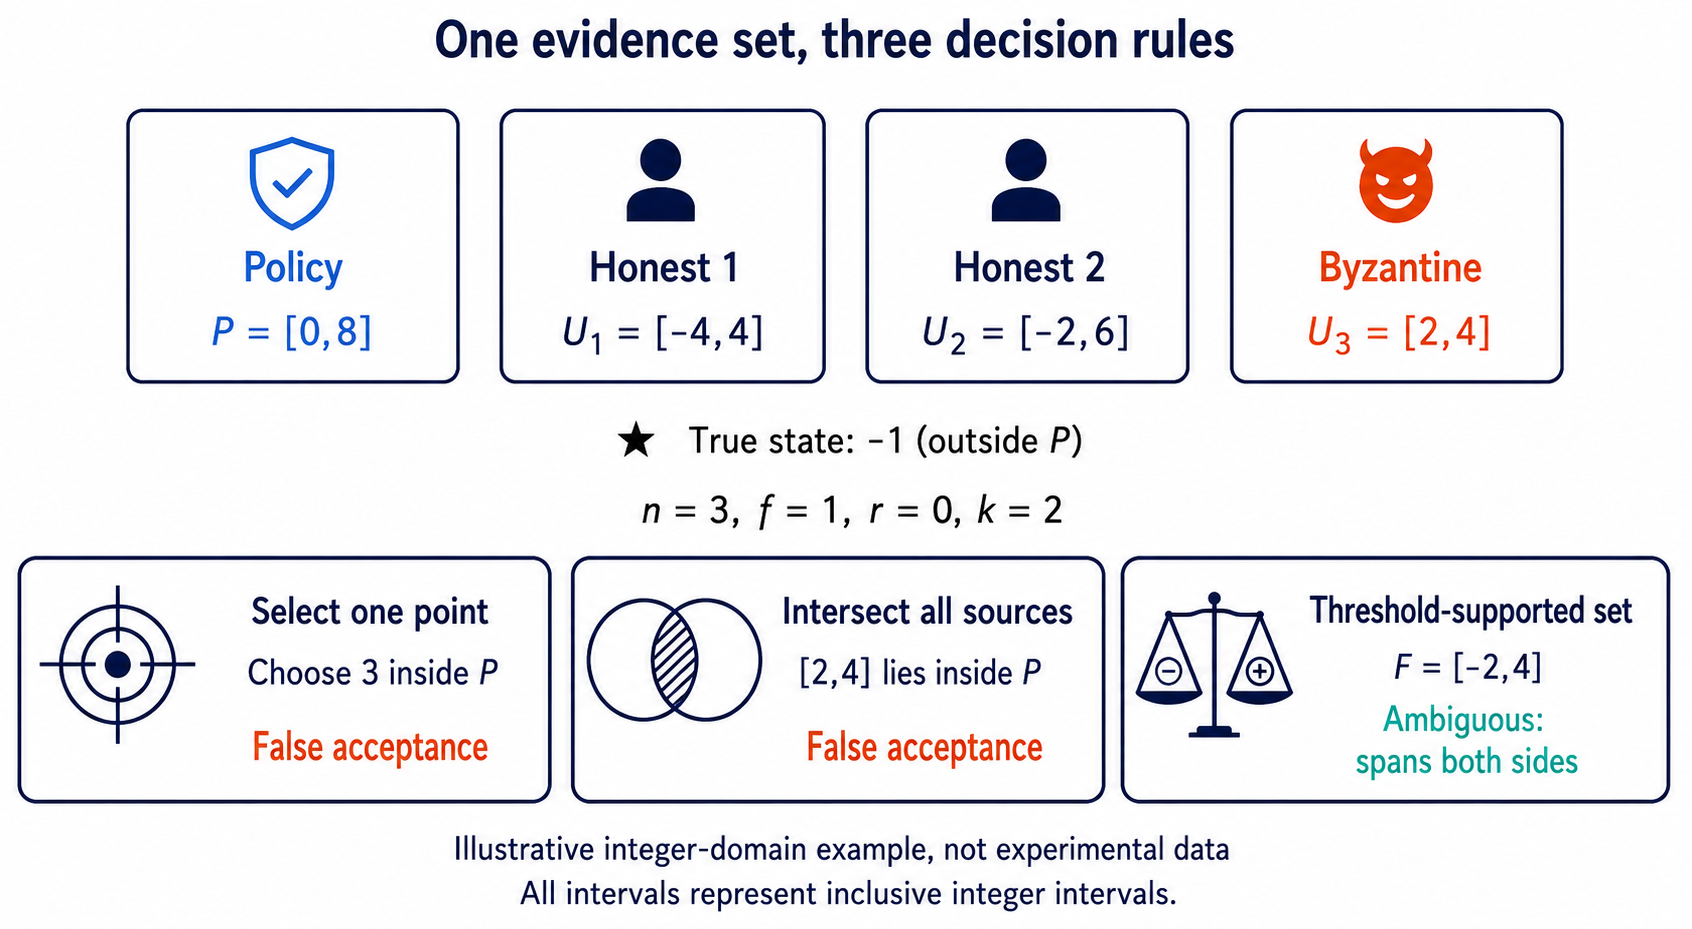
\includegraphics[width=\linewidth]{decision_counterexample.png}
\caption{Three rules applied to the same signed evidence, with inclusive integer intervals and $(n,f,r,k)=(3,1,0,2)$. A selected point or full-source intersection can falsely accept the known noncompliant true state, whereas threshold support yields an ambiguous decision. The example is constructed rather than measured.}\label{fig:counterexample}
\end{figure}

\subsection{Report binding and challenge--response verification}
To prevent a valid geometric proof from being replayed across different reports or tasks, the protocol employs the expiring challenge-response workflow shown in Figure~\ref{fig:sequence}.

An administrator configures the task, verifying key, spacetime policy, threshold, and ordered issuer roster. The gateway retains a trusted snapshot of these settings, verifies that keys and trust-domain labels are unique, and issues a random 256-bit challenge nonce $\nu$ with an expiry timestamp $e$ from its trusted clock. The vehicle and issuers derive a shared context:


\begin{equation}\label{eq:context}
c = \mathrm{OS2IP}(\mathrm{SHA256}(\mathrm{Encode}(\mathrm{ver}, T, \nu, e, \mathrm{SHA256}(R)))) \bmod q.
\end{equation}


Here $\mathrm{ver}$ is the protocol version, $T$ is the configured task, $R$ is the raw report byte sequence, $q$ is the BN254 scalar-field modulus, and $\mathrm{OS2IP}$ maps a byte sequence to an integer. Context $c$ cryptographically binds the signed evidence and proof statement to $R$ and $\nu$ without encrypting $R$. In our implementation, $\mathrm{Encode}(\cdot)$ uses a deterministic Go JSON struct with fixed field ordering, lowercase hexadecimal SHA-256 digests, and Base64-encoded public keys.

Each issuer signs the digest $m_i$ in (2) containing $c$ and its interval bounds. After collecting all roster signatures, the vehicle evaluates the four-valued decision rule and generates a zero-knowledge proof using the interval endpoints and signatures as private witness data. The gateway verifies that $\nu$ exists and remains unexpired, reconstructs the public inputs from its trusted task snapshot and received report $R$, and verifies the proof and decision code, accepting only a verified Valid outcome.

Upon successful verification, the gateway atomically marks $\nu$ as consumed within its active instance. Failed proof verifications leave an unexpired challenge open for legitimate retries.

\paragraph{Availability and task outcomes.} The current all-roster rule deliberately fails closed when an issuer is unavailable: after the collection deadline, the vehicle cannot obtain a certificate for that challenge and must request a fresh challenge and signed observations rather than silently dropping the missing issuer. A verified Valid result admits the report; an Invalid result rejects it under the configured policy. Ambiguous is returned for host-side resensing, a revised authorized task, or manual review, while Inconsistent triggers evidence-quality diagnosis and recollection. In all non-Valid cases the gateway does not accept the report. A future $n$-of-$N$ dynamic-roster extension could use authenticated subset-selection and threshold parameters, but this is not implemented or measured by the current fixed-roster prototype.

\begin{figure}[htbp]\centering
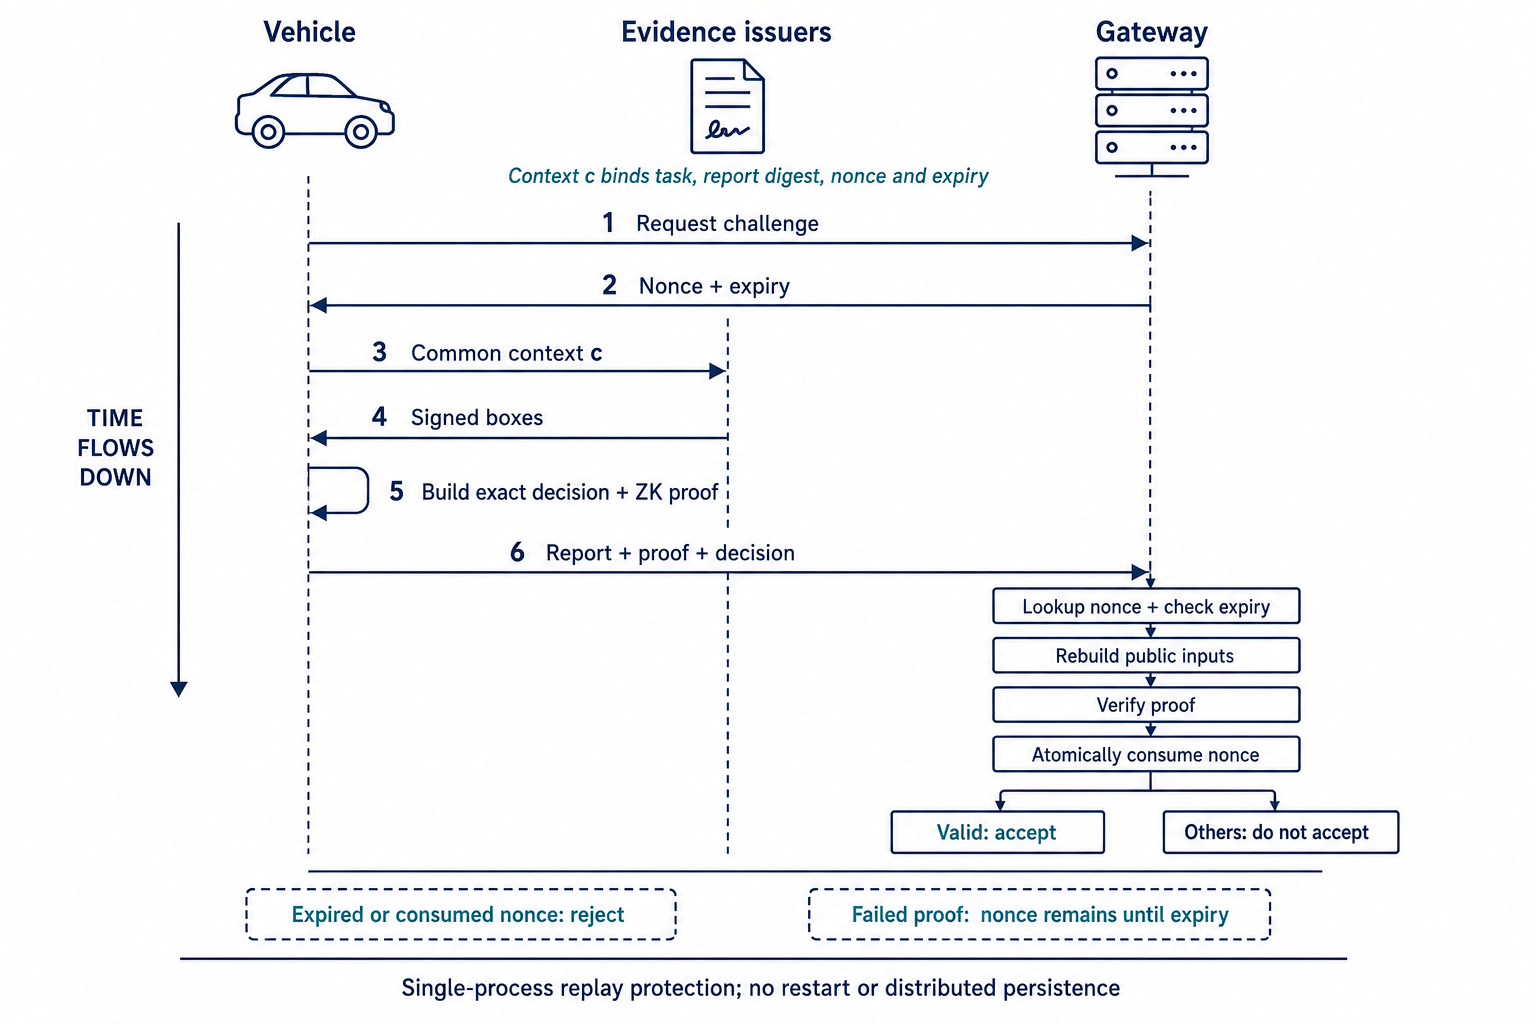
\includegraphics[width=\linewidth]{protocol_sequence.png}
\caption{Report-bound challenge-response and verification workflow. Upon successful proof verification and a Valid decision, the gateway atomically marks the nonce as consumed, whereas failed attempts leave the challenge open for retries until expiry. This schematic was generated with AI assistance (OpenAI ChatGPT); numerical and logical labels require author verification before submission.}\label{fig:sequence}
\end{figure}
\subsection{Zero-knowledge circuit construction}
To certify a four-valued decision without revealing the original observations, the circuit checks signatures, coordinate bounds, and context consistency while determining whether threshold-supported states exist on either side of the policy boundary. We implement two geometric backends: lower-corner maximum-depth reachability and threshold-subset enumeration. Their signature-verification and public-output constraints are shared; they differ in how threshold reachability is calculated.

\subsubsection{Lower-corner maximum-depth reachability}
For a query box $Q\subseteq\Omega$, first clip every evidence box $U_i$ to $Q$. For each axis $a$, let $A_a$ contain the lower endpoints of the nonempty clipped boxes. The following lemma reduces maximum-depth search over the entire query region to a finite candidate set.

\begin{lemma}[Lower-corner maximum-depth reachability]\label{lem:corner}
If the maximum overlap depth inside $Q$ is positive, then some point attaining that depth belongs to $A_1\times\cdots\times A_d$.
\end{lemma}
\begin{proof}
Choose a point $z\in Q$ with maximum depth and let $\mathcal S$ be the collection of clipped boxes containing $z$. Their intersection is nonempty. For each axis $a$, define $v_a$ as the greatest lower endpoint of the boxes in $\mathcal S$. This endpoint belongs to $A_a$. Because $z$ belongs to every box in $\mathcal S$, the greatest lower endpoint on any axis cannot exceed the smallest corresponding upper endpoint. Hence $v=(v_1,\ldots,v_d)$ lies in every box in $\mathcal S$ and has depth at least $|\mathcal S|$, the maximum depth attained by $z$. By maximality, its depth is exactly the same. Thus $v$ is a maximum-depth point in the stated candidate set.
\end{proof}

By the lemma, the circuit enumerates at most $n^d$ lower-corner combinations, including duplicates, and checks both membership in $Q$ and coverage by the signed evidence boxes. A point with coverage at least $k$ exists in $Q$ if and only if an enumerated candidate meets that threshold. A candidate contributed by an interval not intersecting $Q$ cannot automatically be treated as valid: the necessary membership tests still apply.

When $P$ is an axis-aligned integer box, $\Omega\setminus P$ is the union of at most $2d$ axial slabs. Along axis $a$, a lower slab ends at $p_a^- -1$ and an upper slab starts at $p_a^+ +1$; all other axes span the discrete domain. Slabs lying outside $\Omega$ are inactive. The circuit calculates $I$ from reachability in $P$ and $O$ from the disjunction of reachability over complement slabs. It then constrains the public decision code to
\begin{equation}\label{eq:decisioncode}
\delta=(1-I)O+2IO+3(1-I)(1-O).
\end{equation}
For Boolean $I$ and $O$, this expression is exactly the coding in Table~\ref{tab:decisions}. Further constraints check the coordinate bit width, ordering of lower and upper endpoints, and containment of boxes and policy within $\Omega$. EdDSA/MiMC signatures are verified inside the circuit, and issuer public keys are compared for pairwise distinctness using their actual encoded elliptic-curve representations, rather than treating a public key as a single scalar.

\subsubsection{Threshold-subset enumeration and computational cost}
An alternative representation of the robust feasible set is

\begin{equation}\label{eq:subset}
\mathcal{F}_k = \bigcup_{\substack{S \subseteq [n] \\ |S| = k}} \left( \bigcap_{i \in S} U_i \right), \quad [n] = \{1, \dots, n\}.
\end{equation}


The intersection of $k$ axis-aligned integer boxes is either another box or the empty set. Its lower and upper endpoints are obtained via coordinatewise maxima and minima, enabling direct tests for nonemptiness, intersection with $P$, and reachability outside $P$. Both the native reference classifier and the second circuit backend use this exact identity, requiring $O(\binom{n}{k}kd)$ geometric operations.

For a fixed dimension $d$, lower-corner reachability requires $O((2d + 1)dn^{d+1})$ geometric comparisons alongside $n$ signature verifications and $O(n^2)$ pairwise key-distinctness checks, and accepts any admissible threshold $k$ as a dynamic public input without recompilation. In contrast, threshold-subset enumeration fixes $k$ at compile time and constrains it against the public threshold. When the total omission budget $b = n - k = f + r$ is a small constant, its geometric work scales as $O(n^{b+1}d)$, whereas as $k$ approaches $n/2$, the subset count $\binom{n}{k}$ grows combinatorially.

For example, at $(n, d, k) = (5, 3, 4)$, subset enumeration checks $\binom{5}{4} = 5$ intersections, whereas lower-corner reachability evaluates up to $5^3 = 125$ candidates per query region. Using the geometric operation proxies $W_D = (2d + 1)dn^{d+1}$ and $W_S = \binom{n}{k}kd$, we have $W_D = 3,360,000$ versus $W_S = 1,140$ at $(n, d, k) = (20, 3, 19)$; when $k$ decreases to $10$, $W_D$ remains constant while $W_S$ increases to $5,542,680$. Thus, both backends implement the exact same four-valued relation while trading runtime threshold flexibility against geometric circuit size in small-omission regimes.

\section{Security Analysis}\label{sec:security}
Gateway acceptance depends on both cryptographic and physical assumptions. Signatures, context binding, and zero-knowledge proofs constrain the origin of the evidence, its association with a task, and the computed relation. A conclusion about the physical event also requires the honest-source coverage condition. We state the threat model and analyze soundness, protocol attacks, and information leakage below.

\subsection{Threat model and security objectives}
We treat the vehicle and its communication network as untrusted. A computationally bounded adversary may intercept, modify, reorder, or replay reports, proofs, decision codes, and challenge parameters, and may use the private keys of up to $f$ compromised issuers to sign deceptive, policy-aware uncertainty regions. Honest issuers protect their signing keys and bind their observations to the intended event and task context. The gateway's task configuration, verifying key, issuer roster, and clock are trusted, and the underlying signature, hash, and proof primitives satisfy standard computational security assumptions.

We analyze six core security properties---evidence authenticity, context integrity, conditional acceptance soundness, witness confidentiality, challenge freshness, and fail-closed behavior---summarized in Table 3. Here, witness confidentiality protects the private spacetime boxes and signatures from the verifier and external observers, while the business report payload $R$ and task metadata remain visible to the gateway.

\begin{table}[htbp]\centering\footnotesize
\caption{Security properties, prerequisites, and validation.}\label{tab:security-properties}
\begin{tabularx}{\linewidth}{@{}p{0.20\linewidth}p{0.30\linewidth}X@{}}\toprule
Property & Assumptions & Mechanism or observation\\\midrule
Evidence authenticity & Honest keys uncompromised outside the Byzantine allowance; signature unforgeability & In-circuit EdDSA/MiMC verification; modified signed bounds rejected\\
Context integrity & Trusted task configuration; signed-message and context mappings satisfy collision/binding assumptions & Binding to task, report, roster, threshold, nonce and expiry; tested substitutions rejected\\
Conditional acceptance soundness & Sound proof system; at most $f$ Byzantine issuers and $r$ honest misses & Four-valued relation, Propositions~\ref{prop:soundness}--\ref{prop:composition}, and synthetic checks tagged by $M\le r$\\
Witness confidentiality & Zero knowledge of the instantiated proof system; explicit public-output leakage & Box endpoints and signatures remain private witness values; other disclosure is summarized in Table~\ref{tab:privacy-boundary}\\
Freshness & Trusted clock; atomic challenge updates in one gateway instance & Expiry checks and atomic marking after successful verification; one accepted among eight concurrent replays\\
Fail-closed behavior & Correct gateway procedure and complete configured roster & Missing/malformed evidence, mismatched codes, unknown/expired challenges, or duplicated roster entries abort or are rejected\\\bottomrule
\end{tabularx}\end{table}

\subsection{Correctness and conditional soundness}
\begin{proposition}[Conditional evidence soundness]\label{prop:soundness}
Suppose at most $f$ of the $n$ enrolled issuers are Byzantine, and at most $r$ boxes submitted by honest issuers fail to cover the true reference state $z^*$. With $k = n - f - r$, we have $z^* \in \mathcal{F}_k$. Consequently, a Valid decision entails $z^* \in P$, and an Invalid decision entails $z^* \notin P$.
\end{proposition}
\begin{proof}
At least $n - f - r = k$ honest boxes contain $z^*$. By the definition of the feasible set in (3), its coverage depth at $z^*$ is at least $k$, so $z^* \in \mathcal{F}_k$. A Valid decision requires $\emptyset \neq \mathcal{F}_k \subseteq P$, implying $z^* \in P$, whereas an Invalid decision requires $\mathcal{F}_k \cap P = \emptyset$, implying $z^* \notin P$.
\end{proof}

If the stronger condition $n > 2f + r$ holds, then $k > f$, ensuring that every state in $\mathcal{F}_k$ is supported by at least one honest issuer; however, $k = n - f - r \ge 1$ suffices to guarantee $z^* \in \mathcal{F}_k$.

To quantify the probability that honest miscoverage exceeds the allowance $r$, let $\mathcal{H}$ denote the set of honest issuers, and let $M$ count the honest boxes that miss $z^*$. If each honest issuer $i \in \mathcal{H}$ has marginal miss probability at most $\alpha_i$, Markov's inequality yields a distribution-free upper bound that holds even under arbitrarily correlated errors:


\begin{equation}\label{eq:calibration}
\Pr(M > r) = \Pr(M \ge r + 1) \le \min\left\{ 1, \frac{\sum_{i \in \mathcal{H}} \alpha_i}{r + 1} \right\}.
\end{equation}

The gateway acceptance guarantee also depends on cryptographic soundness. Under the knowledge soundness of Groth16 (given a secure circuit-specific setup), an accepted proof guarantees the existence of a witness satisfying all signature, range, and geometric constraints. Combined with EdDSA unforgeability and the collision/binding resistance of the MiMC prehash and context mapping, this witness must correspond to authenticated intervals bound to the designated task and report.

\begin{proposition}[Gateway acceptance under physical coverage]\label{prop:gateway}
Assume an authorized task configuration and roster, a trustworthy gateway procedure and clock, unforgeable honest-issuer signatures, a knowledge-sound proof system, and collision-resistant MiMC and context bindings. If the gateway accepts a report and the fault and coverage premises of Proposition 1 hold, then the report-bound reference event $z^*$ satisfies $z^* \in P$, up to negligible cryptographic failure probabilities.
\end{proposition}
\begin{proof}
The gateway reconstructs the public statement from its trusted task snapshot and received report bytes, accepting only a verified proof with decision code Valid. By knowledge soundness, signature unforgeability, and context binding, verification guarantees the existence of authenticated boxes satisfying $\emptyset \neq \mathcal{F}_k \subseteq P$ for the current context. Under the physical coverage premise, Proposition 1 yields $z^* \in \mathcal{F}_k \subseteq P$.
\end{proof}

To formalize the composition of cryptographic and physical premises, let $\mathsf{Acc}$ denote gateway acceptance, $\mathsf{Cov}$ denote the event that the Byzantine ($f$) and honest-miscoverage ($r$) budgets hold, and $\mathsf{Comp}$ denote $z^* \in P$. For a given adversary and security parameter, let $\epsilon_{\mathrm{snark}}, \epsilon_{\mathrm{sig}}, \epsilon_{\mathrm{MiMC}}, \epsilon_{\mathrm{ctx}}$, and $\epsilon_{\mathrm{state}}$ upper-bound the failure probabilities of proof knowledge soundness, signature unforgeability, MiMC prehash binding, context binding, and challenge-state enforcement, respectively.

\begin{proposition}[Composed conditional acceptance bound]\label{prop:composition}
Under a trusted task configuration, roster, and gateway clock, the probability of false acceptance under valid physical coverage satisfies

\begin{equation}\label{eq:composed}
\Pr[\mathsf{Acc} \wedge \mathsf{Cov} \wedge \neg\mathsf{Comp}] \le \epsilon_{\mathrm{snark}} + \epsilon_{\mathrm{sig}} + \epsilon_{\mathrm{MiMC}} + \epsilon_{\mathrm{ctx}} + \epsilon_{\mathrm{state}}.
\end{equation}
\end{proposition}
\begin{proof}
If none of the five cryptographic or state-enforcement failure events occurs, an accepted proof ensures $\emptyset \neq \mathcal{F}_k \subseteq P$ for the authentic task and report context. Under $\mathsf{Cov}$, Proposition 1 implies $z^* \in \mathcal{F}_k \subseteq P$ ($\mathsf{Comp}$). Thus, $\mathsf{Acc} \wedge \mathsf{Cov} \wedge \neg\mathsf{Comp}$ implies at least one failure event, and the union bound gives (8).
\end{proof}

In a single-process gateway with atomic nonce consumption, replay of an already accepted challenge has $\epsilon_{\mathrm{state}} = 0$. The prototype instantiates these primitives with 256-bit nonces, SHA-256 context hashing, Groth16 over BN254, and gnark's twisted-Edwards BN254 EdDSA/MiMC implementation.

\subsection{Resistance to protocol attacks}
\textbf{Evidence tampering and context substitution.} Modifying any endpoint of a signed region $U_i$ alters its MiMC digest in (2), causing in-circuit EdDSA verification to fail unless the adversary forges an honest issuer's signature. Similarly, substituting the task, report bytes, roster, threshold, challenge nonce, or expiry alters the public context $c$ reconstructed by the gateway, invalidating proofs generated for prior statements. Missing signatures, duplicated roster keys, or mismatched decision codes trigger immediate gateway rejection or protocol abort rather than producing a certified Inconsistent outcome.

\textbf{Challenge replay.} The gateway mitigates replay attacks by verifying challenge existence and expiry prior to proof checking and atomically marking the nonce as consumed upon Valid acceptance. Consequently, concurrent submissions of an identical valid request succeed at most once within the gateway instance. Because failed verifications do not consume unexpired nonces, legitimate provers can retry after transient errors, while deployment-level rate limiting can be applied to throttle repeated invalid submissions.

\textbf{Policy-aware Byzantine intervals.} Compromised issuers may craft intervals strategically using full knowledge of the public policy $P$. Provided the fault and miscoverage budgets ($f$ and $r$) hold, Proposition 1 ensures $z^* \in \mathcal{F}_k$ regardless of adversarial box placement. Thus, a noncompliant event ($z^* \notin P$) cannot yield $\mathcal{F}_k \subseteq P$ (Valid), and a compliant event ($z^* \in P$) cannot yield $\mathcal{F}_k \cap P = \emptyset$ (Invalid). Strategic Byzantine boxes can at most expand $\mathcal{F}_k$ across the boundary to induce an Ambiguous outcome or withhold signatures to force an abort, but cannot induce a wrong decisive classification.

\subsection{Privacy boundary and information leakage}
Zero-knowledge proofs allow the gateway to verify the four-valued compliance relation without learning the private witness (the signed intervals $U_i$ and their signatures). Table~\ref{tab:privacy-boundary} delineates the visibility boundaries across protocol roles. Because the gateway receives the plaintext report $R$ to reconstruct the deterministic binding context $c$, $c$ acts as an integrity commitment rather than a hiding commitment; for low-entropy reports, an external observer who knows the task and challenge parameters could mount an offline dictionary test against $c$.

\begin{table}[htbp]\centering\footnotesize
\caption{Visibility and leakage boundaries for protocol participants.}\label{tab:privacy-boundary}
\begin{tabularx}{\linewidth}{@{}p{0.19\linewidth}p{0.37\linewidth}X@{}}\toprule
Role & Visible within the protocol model & Not concealed by the ZK guarantee\\\midrule
Evidence issuer & Its own observation and region, signing operation, and report-bound context & Its own evidence and any report data supplied by the host application\\
Vehicle/prover & Report, regions, and signatures required to build the witness & Secrecy of the witness from the prover itself is not an objective\\
Gateway/verifier & Report bytes, task/domain, policy, threshold, roster, nonce/expiry, public context, proof, classification & Report content, public policy, issuer identities, classification\\
Public transcript observer & Exposed statement, proof, classification, and transport metadata & Linkability of public fields and offline candidate tests for low-entropy reports\\\bottomrule
\end{tabularx}\end{table}

The distinction between revealing a two-bit output symbol and leaking the underlying witness is important: the entropy bound describes the size of the output alphabet, not a measured mutual-information leakage about the location.

Furthermore, the public four-valued classification $\delta \in \{0, 1, 2, 3\}$ inherently reveals up to $\log_2 4 = 2$ bits of information per query (and an upper bound of $2q$ bits on the joint output alphabet over $q$ queries, without implying additive information leakage about the witness) regarding the relationship between $\mathcal{F}_k$ and $P$. While a single task-bound check preserves witness confidentiality within the authorized region, unrestricted adaptive policy queries could progressively narrow the candidate location space, motivating query-authorization and rate-control policies in multi-query applications.
\section{Experimental Evaluation}
We evaluate the proposed evidence-certification framework across three dimensions: protocol security regressions, four-valued decision semantics under synthetic and trajectory-replay workloads, and Groth16 cryptographic performance across both circuit backends.

\subsection{Implementation and experimental setup}
\subsubsection{Cryptographic implementation and test environment}
The prototype is implemented in Go 1.25.6 using \texttt{gnark} v0.14.0 ~\citep{gnark}, Groth16 over BN254 ~\citep{Groth2016}, and \texttt{gnark}'s twisted-Edwards BN254 EdDSA and MiMC primitives for in-circuit signature verification ~\citep{MiMC2016}. Key generation, signing, setup, proving, and verification all execute full cryptographic operations. The source code and benchmark scripts are organized under \texttt{prototype/} and \texttt{experiments/} in our open-source repository.

Proof benchmarks were conducted on a Mac mini equipped with an 8-core Apple M1 processor and 16 GB of RAM. For each circuit configuration, we performed one setup followed by 30 proof generation and verification trials over a valid signed witness, measuring pure proving and verification kernel latencies. As a structural reference for baseline geometric overhead, we also implemented a simplified hidden-point region-membership circuit on the same \texttt{gnark}/Groth16/BN254 stack (omitting issuer signatures, threshold fusion, and four-valued logic).

To evaluate circuit scalability separately from proving latency, we compiled full signed-evidence R1CS instances across issuer counts $n \in \{4, 8, 12, 16\}$ and dimensions $d \in \{2, 3\}$. For each $(n, d)$ pair, we tested subset enumeration with $k = n - 1$, $k = n - 2$, and $k = n/2$, alongside lower-corner reachability (32 compilations in total), enforcing a 30 s timeout, a 3 GiB resident set size (RSS) cap, and a 2500 MiB Go soft memory target.

\subsubsection{Synthetic evidence and trajectory replay}
The semantic evaluation uses the 3D integer domain $\Omega = [0, 63]^3$ and policy $P = [18, 45]^3$ with $n = 5$ issuers, Byzantine budget $f = 1$, and baseline miscoverage allowance $r = 0$. We cross maximum uncertainty radii $\{2, 4, 6\}$, actual Byzantine counts $\{0, 1, 2\}$, and three error models (independent calibrated, correlated calibrated, and undercovered) to form 27 conditions. Each condition runs 30 random seeds with 80 events per seed (64,800 base observations), placing 75\% of events near policy boundaries. Byzantine issuers select intervals adversarially using the true state $z^*$ and policy $P$.

We compare the robust feasible-set rule against four baselines specified below: median point claim, majority-center voting, fixed maximum-radius margin, and all-source intersection. False acceptance (FA) and false rejection (FR) are \emph{marginal rates}: $\mathrm{FA}=\#\{\mathrm{Valid}\wedge z^*\notin P\}/\#\{z^*\notin P\}$ and $\mathrm{FR}=\#\{\mathrm{Invalid}\wedge z^*\in P\}/\#\{z^*\in P\}$. Their denominators include ambiguous and evidence-failure outcomes, and are not conditioned on producing a decisive classification. Decisive coverage is $\#\{\mathrm{Valid},\mathrm{Invalid}\}/N$; wrong-among-decisive risk instead divides false decisions by the number of decisive decisions. Because the circuit backends and the native reference classifier are mathematically identical over $\Omega$ (verified via randomized equivalence tests), the large-scale semantic sweeps execute the native classifier directly, while Groth16 proving costs are benchmarked in Section~\ref{sec:crypto-perf}. Each event logs the number $M$ of honest intervals missing $z^*$ to track satisfaction of Proposition 1's premise ($M \le r$), and all 64,800 observations are re-evaluated across $r \in \{0, 1, 2\}$ in paired ablation tests.

To evaluate realistic vehicle kinematics, we extract 787 measured reference states (spanning 786 s) from the UrbanNav-HK-Medium-Urban-1 dataset ~\citep{UrbanNav}. In a local integer frame, a policy $P$ using the 20th and 80th percentiles of each locally quantized coordinate encloses 169 states. Across 30 replay seeds, we simulate four honest sources with bounded correlated errors and one policy-aware Byzantine source along the measured trajectory, plus a stress regime that multiplies the shared common-mode innovation by four (from $1\times$ to $4\times$), with 0.9 autoregressive persistence.


\subsubsection{Synthetic evidence generator and baseline definitions}
The generator is fixed by the released experimental script and evaluated without per-condition parameter tuning. For each of 30 seeds (integer base seed 20260904), it samples 80 events for every condition. In 75\% of events, one randomly chosen coordinate is placed within $[-(a+1),a+1]$ of a randomly chosen policy face, where $a$ is the maximum radius; the remaining events are uniformly sampled from $\Omega$. For each honest issuer, the integer box half-width $h$ is sampled uniformly from $\{\max(1,\lfloor a/2\rfloor),\ldots,a\}$ and independently for each source; the observed center is clipped to $\Omega$, and the inclusive uncertainty box is the center plus/minus $h$ clipped to the domain.

For independent calibrated errors, the three integer center offsets are each uniform on $[-h,h]$. For correlated calibrated errors, a shared direction $s\sim\mathrm{Uniform}([-1,1]^3)$ is sampled per event and the center offset is $\mathrm{clip}_{[-h,h]}(\mathrm{round}((0.75s+\eta)h))$, where $\eta_a\sim\mathrm{Uniform}[-0.20,0.20]$ independently for each issuer and coordinate. Undercoverage uses $\mathrm{round}((1.35s+\eta')h)$, with $\eta'_a\sim\mathrm{Uniform}[-0.15,0.15]$, without clipping the offset to the declared $h$. These are constructive common-mode error models, not a measured correlation coefficient or an assumed parametric GNSS error distribution.

The Byzantine strategy is policy-aware but deterministic. If the true state lies outside $P$, each compromised issuer signs exactly the public policy box $P$, encouraging false acceptance under naive intersection. If the true state lies in $P$, the adversary selects the nearest available policy face and signs a domain-wide slab immediately outside that face, encouraging false rejection. Compromised boxes are then shuffled among the honest boxes. Table~\ref{tab:generator} lists the exact parameter grid; the 12 within-budget conditions use the two calibrated models, three radii, and zero or one actual Byzantine issuer. The remaining 15 conditions are retained as assumption stress tests (nine undercovered-model settings and six calibrated-model settings with two compromised issuers). The admissible calibrated cases have $M=0$ for each honest source by construction.

\begin{table}[htbp]\centering\footnotesize
\caption{Synthetic generator parameters, held fixed across baseline methods.}\label{tab:generator}
\begin{tabularx}{\linewidth}{@{}p{0.33\linewidth}X@{}}\toprule
Parameter & Implemented setting\\\midrule
Integer domain and policy & $\Omega=[0,63]^3$, $P=[18,45]^3$\\
Sources and verifier budgets & $n=5$, $f=1$, baseline $r=0$ ($k=4$)\\
Grid, seeds, events & Maximum radius $a\in\{2,4,6\}$; actual Byzantine count $0,1,2$; three error models; 30 seeds; 80 events per condition (27 conditions, 64,800 events)\\
Source radius & Integer $h\sim\mathrm{Unif}\{\max(1,\lfloor a/2\rfloor),\ldots,a\}$\\
Independent calibrated & $e_a\sim\mathrm{Unif}\{-h,\ldots,h\}$\\
Correlated calibrated & $e=\mathrm{clip}(\mathrm{round}[(0.75s+\eta)h],-h,h)$; $s\sim U[-1,1]^3$, $\eta_a\sim U[-0.20,0.20]$\\
Undercovered correlated & $e=\mathrm{round}[(1.35s+\eta')h]$, $\eta'_a\sim U[-0.15,0.15]$; no offset clipping\\
Byzantine evidence & $U_i=P$ if $z^*\notin P$; otherwise a domain-wide slab directly outside the nearest available policy face\\
Boundary sampling & 75\% within $a+1$ integer cells of a randomly selected policy face; 25\% uniform\\\bottomrule
\end{tabularx}\end{table}

The four baselines operate on the same signed-box realizations. \emph{Median point claim} declares Valid exactly when the coordinate-wise median of the box centers lies in $P$, and Invalid otherwise. \emph{Majority-center voting} declares Valid when strictly more than $n/2$ individual box centers lie in $P$, and Invalid otherwise. \emph{Fixed maximum-radius margin} centers a guard box at the coordinate-wise median center with half-width $a$ on every axis (using floor/ceiling integer bounds), and applies the same set-level Valid/Invalid/Ambiguous policy rule to the guard box; $a$ is fixed by the condition, not optimized on the test data. \emph{All-source intersection} applies that policy rule to $\bigcap_i U_i$, returning evidence failure if the intersection is empty. The competing methods are operational baselines, not cryptographic implementations of those rules.

\subsection{Protocol-security regression tests}
Table~\ref{tab:security-validation} summarizes the adversarial regression tests executed against the end-to-end proof and gateway pipeline across mutated evidence bounds, decision codes, task contexts, rosters, and challenge nonces. The tests rejected modified signed interval endpoints and proofs transplanted across tasks or reports. Missing roster signatures caused the protocol to abort rather than return a certified inconsistent decision. In the eight-way concurrent replay test, the atomic state update allowed exactly one copy of the valid request to succeed.

\begin{table}[htbp]\centering\small
\caption{Adversarial regression tests of proof generation and gateway verification.}\label{tab:security-validation}
\begin{tabularx}{\linewidth}{@{}p{0.22\linewidth}p{0.35\linewidth}X@{}}\toprule
Attack & Enforced constraint & Observed prototype response\\\midrule
Evidence-bound tampering & Signed interval endpoints, issuer slot, context & Altered signed bounds were rejected\\
Decision substitution & Agreement between four-valued circuit output and public decision code & Tested mismatched proof/code pairs were rejected\\
Task or report substitution & Binding to task, report, threshold, roster, nonce and expiry & Tested cross-context substitutions were rejected\\
Challenge replay & Expiry and atomic state update after successful verification & Unknown or expired nonces were rejected; one of eight concurrent copies succeeded\\
Roster manipulation & Distinct ordered keys and trust-domain labels & Duplicated keys or labels were rejected\\
Missing issuer evidence & Complete evidence from the provisioned roster is required & Protocol aborted rather than certifying inconsistency\\\bottomrule
\end{tabularx}\end{table}
\subsection{Robustness and baseline comparison}
Across the 12 synthetic conditions where the actual Byzantine count and honest coverage satisfy the configured budgets ($f$ and $r$), the robust feasible-set rule achieved zero wrong decisive classifications (0\% FA and 0\% FR) with a mean decisive coverage of 87.52\%, outperforming the fixed-margin baseline (75.63\%) by 11.89 percentage points. A paired cluster bootstrap resampling the 12 condition-level differences with replacement (20,000 draws; fixed pseudorandom seed 718263) yields a 95\% percentile interval of [9.45, 14.56] percentage points. Across these conditions, robust decisive coverage ranges from 79.46\% to 94.29\%, versus 62.63\% to 85.96\% for the fixed-margin baseline. The 11.89-point result is a macro-average over 12 calibrated conditions; the 9.38-point gain reported next is specific to the correlated, radius-four, one-Byzantine focus condition.

\begin{table}[htbp]\centering\footnotesize
\caption{Decisive coverage across the 12 within-budget synthetic conditions (percent). Values are means over 30 seeds per condition; each condition comprises 2,400 events.}\label{tab:twelve}
\begin{tabular}{lrrrr}\toprule
Honest error model&$a$&Actual Byzantine&Robust&Fixed margin\\\midrule
Independent&2&0&94.29&85.21\\
&2&1&94.00&83.42\\
&4&0&90.50&76.38\\
&4&1&87.50&72.58\\
&6&0&85.96&68.83\\
&6&1&84.96&62.62\\
Correlated&2&0&92.04&85.96\\
&2&1&91.25&85.58\\
&4&0&85.08&75.54\\
&4&1&85.04&75.67\\
&6&0&79.46&67.54\\
&6&1&80.12&68.25\\
\bottomrule
\end{tabular}\end{table}




Table~\ref{tab:semantic} details the focus condition (correlated calibrated errors, maximum radius 4, and one Byzantine issuer). The robust rule achieves 85.04\% decisive coverage with zero errors, whereas the fixed-margin rule reaches 75.67\%. Point-estimation baselines (median point and majority center) classify 100\% of events but suffer from 2.10\% FA and 15.29\%--16.30\% FR due to boundary uncertainty. All-source intersection fails on 87.63\% of events and has a marginal 8.64\% FA among truly outside events and 47.55\% FR among truly inside events. Among its rare decisive classifications, all observed decisions in the focus sample were wrong; reporting only marginal rates would obscure this selectivity. Using a 10,000-resample paired bootstrap across the 30 seed groups, the robust rule improves decisive coverage over fixed margins by 9.38 percentage points (95\% CI: $[8.25, 10.54]$ percentage points).



\begin{table}[htbp]\centering\small
\caption{Focus-condition classification results: means over 30 seeds of 80 events each (percent). FA/FR use outside/inside denominators; the other columns use all events.}\label{tab:semantic}
\begin{tabular}{lrrrrr}\toprule
Method&FA&FR&Amb.&Failure&Decisive\\\midrule
Median point claim&2.10&15.29&0&0&100\\
Majority center&2.10&16.30&0&0&100\\
Fixed maximum-radius margin&0&0&24.33&0&75.67\\
All-source intersection&8.64&47.55&0&87.63&12.38\\
Robust feasible set&0&0&14.96&0&85.04\\\bottomrule
\end{tabular}\end{table}

Grouping events by the actual honest-miscoverage count $M$ checks Proposition 1 against the simulated cases. In the focus condition, all 2,400 events satisfy $M = 0 \le r$ with zero observed wrong decisive outcomes. At the seed-group level, the 30 independent seeds yield a one-sided 95\% exact binomial upper bound of 9.50\% on the probability that a seed exhibits at least one wrong decisive outcome; this does not establish a zero population error rate. Under the undercovered error model, the proportion of events satisfying $M \le r$ increases from 52.42\% ($r = 0$) to 62.79\% ($r = 1$) and 73.42\% ($r = 2$). Across all three settings, events satisfying $M \le r$ incurred strictly zero wrong decisive classifications, whereas premise violations ($M > r$) resulted in wrong-decisive rates of 1.31\%, 0.67\%, and 0.47\%, respectively.

\begin{figure}[htbp]\centering
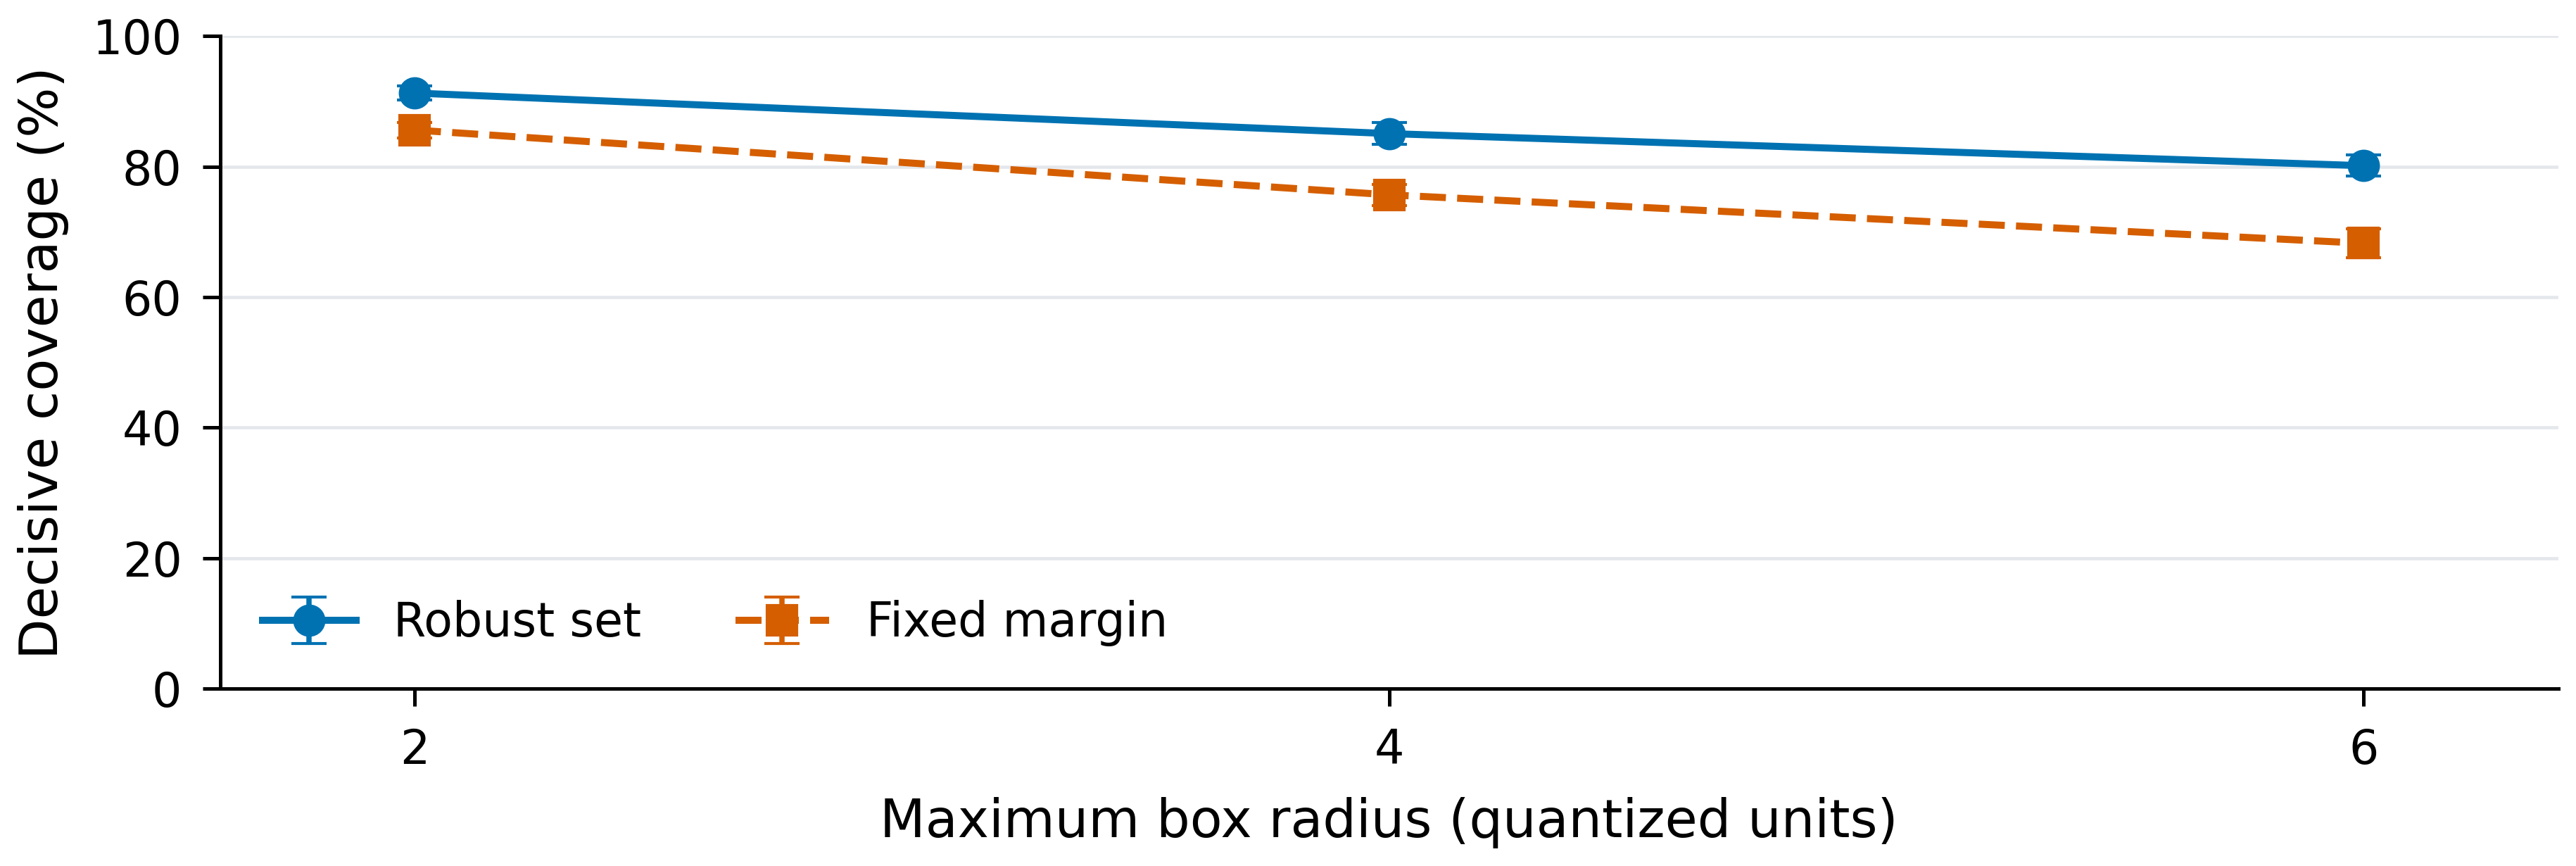
\includegraphics[width=\linewidth]{availability.png}
\caption{Decisive coverage versus maximum uncertainty radius (in quantized units) under correlated calibrated errors with one Byzantine issuer. Error bars denote 95\% confidence intervals across 30 seeds.}\label{fig:availability}
\end{figure}


Figure~\ref{fig:riskcoverage} presents the corresponding risk--coverage operating points for the focus setting. The plotted conditional risk divides wrong decisive outcomes by all decisive classifications, unlike the marginal FA/FR definitions in Table~\ref{tab:semantic}. Since each baseline is tested at one fixed operating point, the figure is an operating-point comparison rather than a continuously tuned risk--coverage curve. For example, all-source intersection achieves only 12.38\% coverage and its 297 decisive decisions are all wrong in the aggregate focus sample; the robust and fixed-margin rules both have zero observed risk at different coverage levels.
\begin{figure}[htbp]\centering
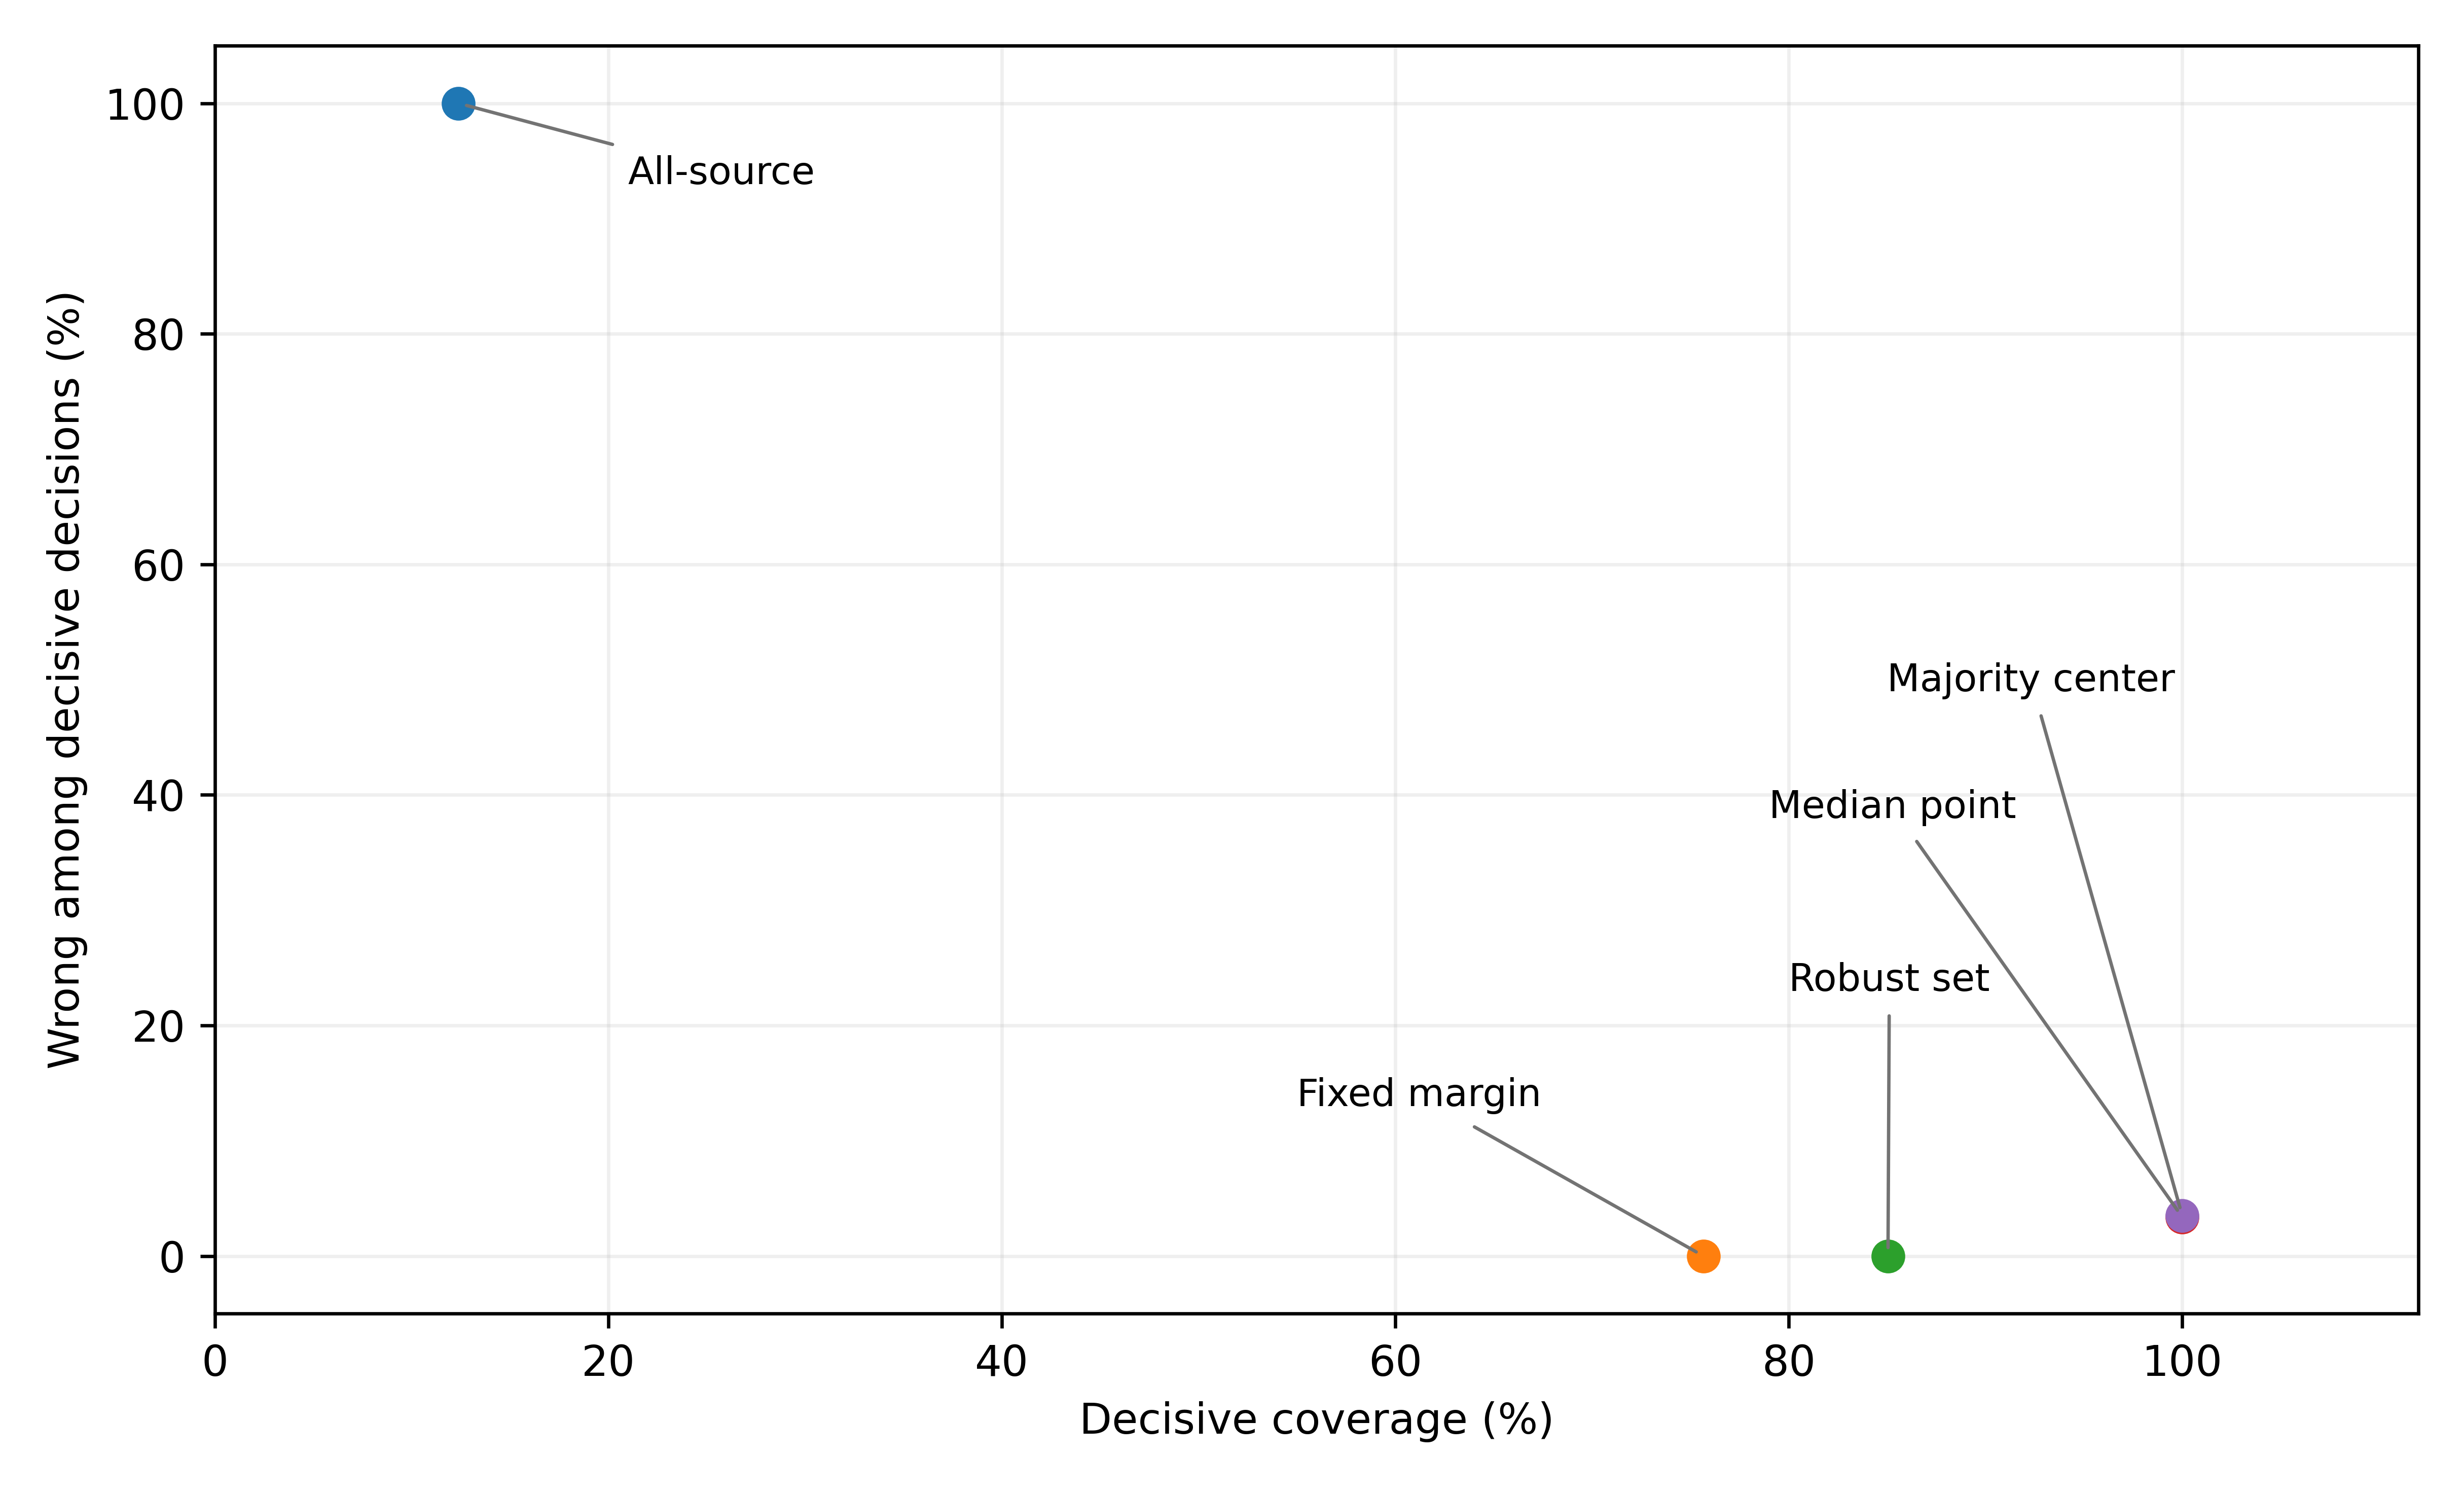
\includegraphics[width=0.92\linewidth]{risk_coverage.png}
\caption{Focus-condition conditional wrong-decision risk versus decisive coverage for five methods; each point uses the aggregate 2,400 generated events. Marginal FA/FR in Table~\ref{tab:semantic} have different denominators.}\label{fig:riskcoverage}
\end{figure}

\subsection{Ablation and out-of-budget stress tests}
Table~\ref{tab:assumption-stress} evaluates system behavior when external assumptions are violated. Under honest-source undercoverage ($M > r$) with one Byzantine issuer, the robust rule experiences 0.23\% FA and 3.41\% FR. When two Byzantine issuers attack a verifier configured for $f = 1$, evidence failure rises to 83.33\% and conditional FA/FR reach 11.62\% and 60.86\%, confirming that the Inconsistent state ($\mathcal{F}_k = \emptyset$) reflects empty threshold support rather than serving as a universal detector for out-of-budget collusion.



\begin{table}[htbp]\centering\small
\caption{Stress conditions violating source assumptions: means over 30 seeds (percent).}\label{tab:assumption-stress}
\begin{tabularx}{\linewidth}{@{}Xrrrr@{}}\toprule
Condition&FA&FR&Evidence failure&Decisive\\\midrule
Honest undercoverage; Byzantine count within budget&0.23&3.41&0&84.92\\
Two actual Byzantine issuers with verifier budget $f=1$&11.62&60.86&83.33&16.67\\\bottomrule
\end{tabularx}\end{table}

Table~\ref{tab:miscoverage} and Figure~\ref{fig:budget} show the paired ablation over the honest-miscoverage budget $r \in \{0, 1, 2\}$ for $n = 5, f = 1$. Because increasing $r$ lowers the support threshold $k = n - f - r$ and expands $\mathcal{F}_k$, it trades decisive coverage for stronger protection against uncalibrated honest misses. Under calibrated evidence, increasing $r$ from 0 to 2 reduces decisive coverage from 85.04\% to 77.46\% while maintaining zero errors. Under undercovered evidence, raising $r$ from 0 to 2 eliminates FA (from 0.23\% to 0\%) and reduces FR from 3.41\% to 0.94\%, with decisive coverage shifting from 84.92\% to 78.50\%.

The UrbanNav trajectory replay shows a similar pattern under simulated multisource errors. Under nominal simulated errors, the robust rule achieves 93.27\% decisive coverage with zero errors, outperforming fixed margins (81.94\%) and avoiding the errors of the median-point baseline (0.29\% FA, 3.12\% FR). Under the $4\times$ common-mode bias stress test, the robust rule maintains low error rates of 0.032\% FA and 0.493\% FR.

\begin{table}[htbp]\centering\small
\caption{Paired ablation over honest-miscoverage allowance ($n=5$, $f=1$, maximum radius four, one Byzantine issuer; percent).}\label{tab:miscoverage}
\begin{tabular}{lrrrr}\toprule
Error model&$r$&FA&FR&Decisive coverage\\\midrule
Calibrated&0&0&0&85.04\\
Calibrated&1&0&0&81.25\\
Calibrated&2&0&0&77.46\\
Undercovered&0&0.23&3.41&84.92\\
Undercovered&1&0&1.79&81.67\\
Undercovered&2&0&0.94&78.50\\\bottomrule
\end{tabular}\end{table}

\begin{figure}[htbp]\centering
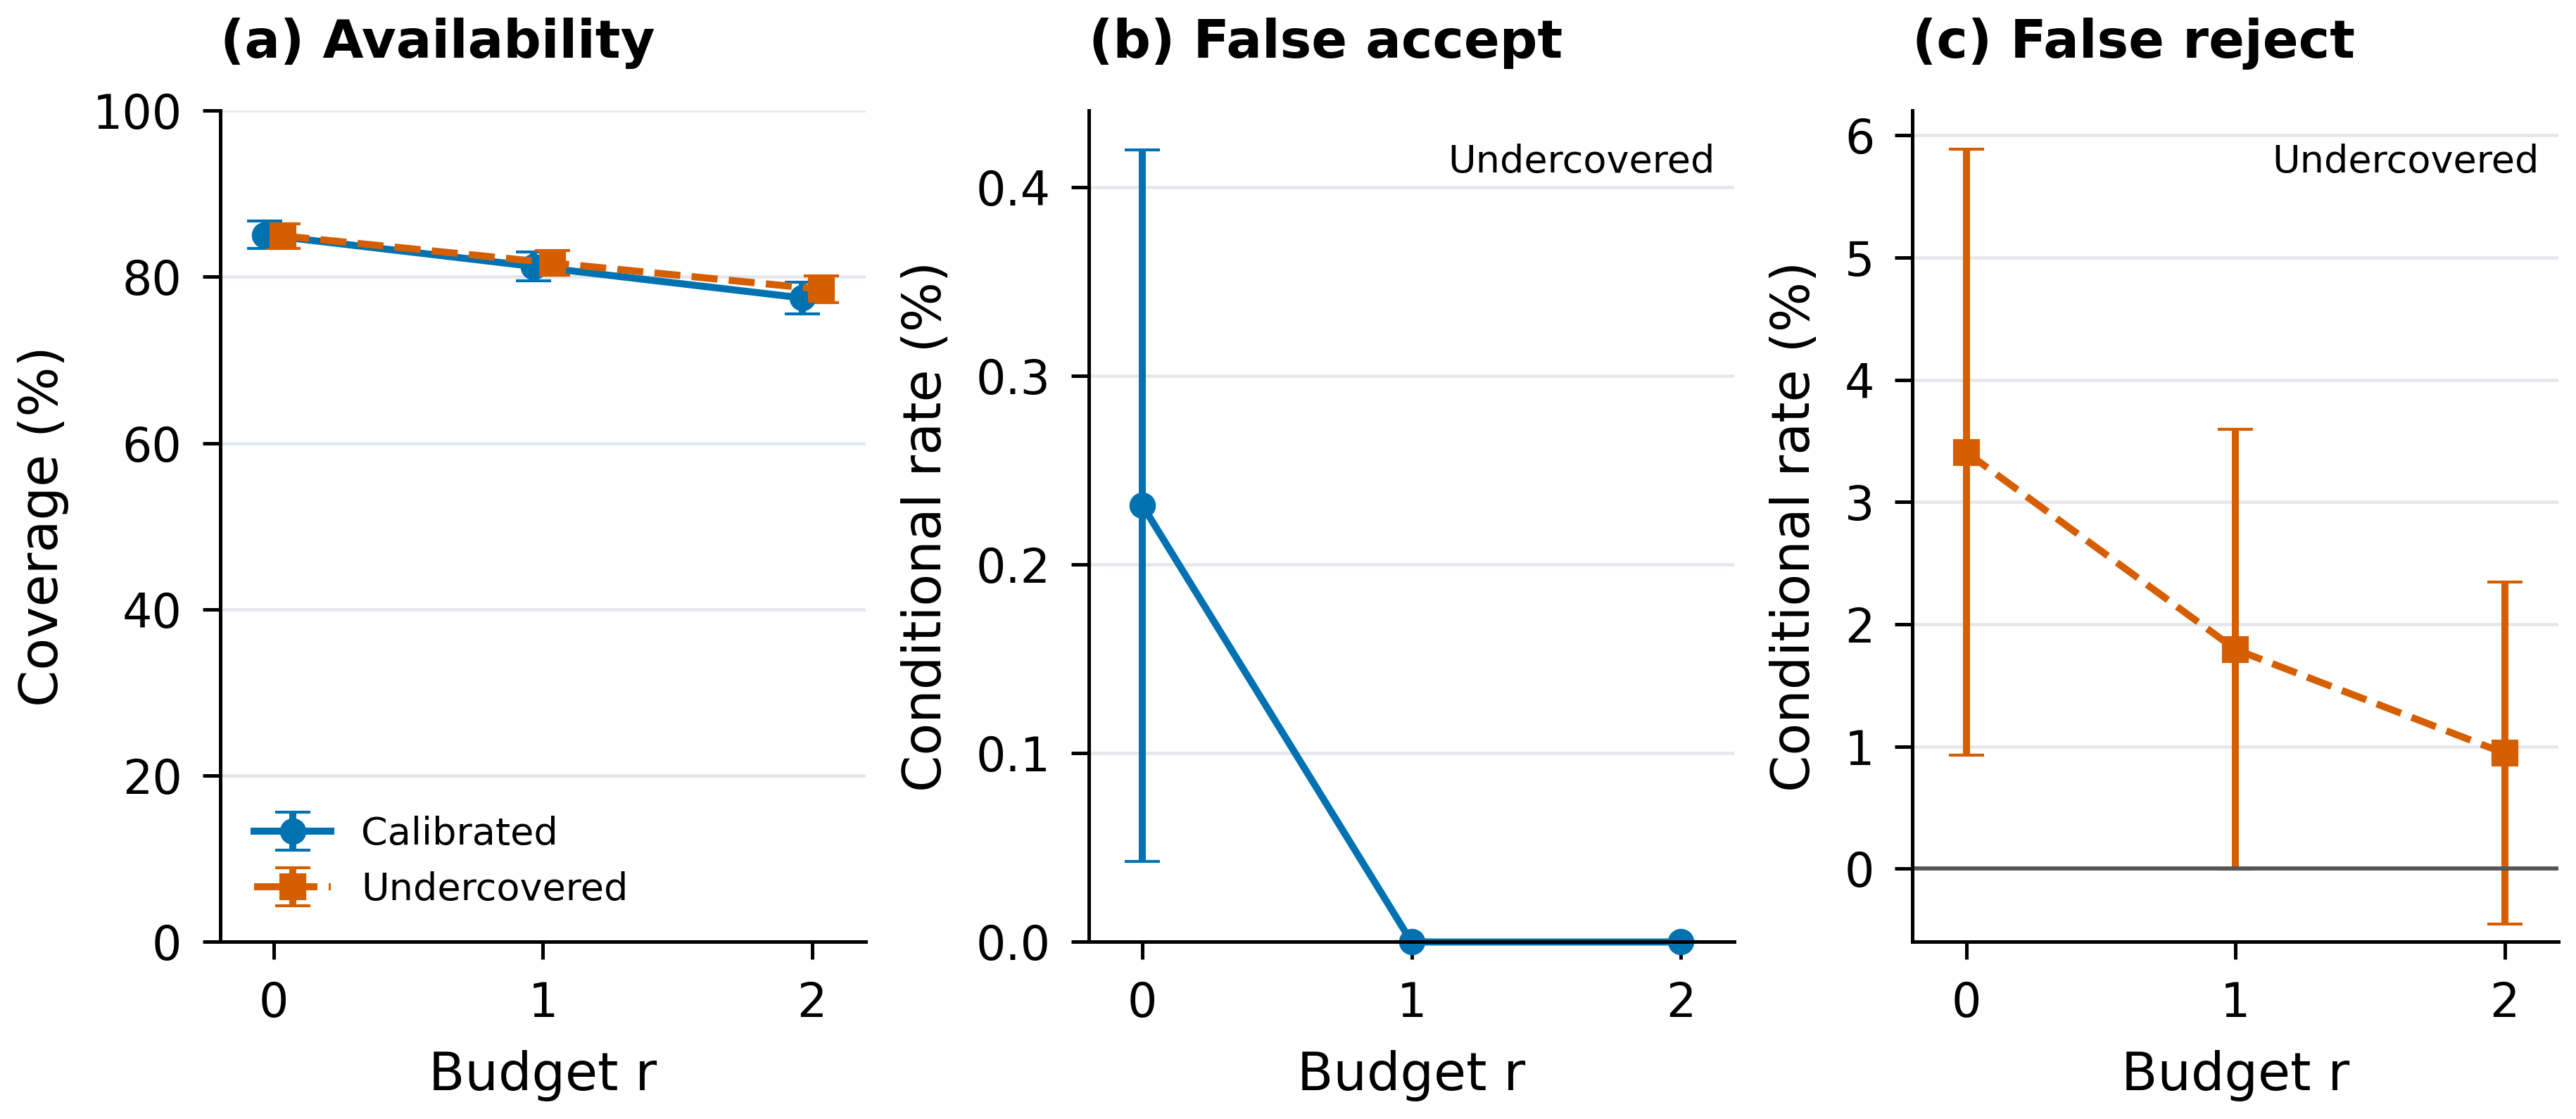
\includegraphics[width=\linewidth]{budget_tradeoff.png}
\caption{Paired ablation over the honest-miscoverage allowance $r$ for $n = 5, f = 1$: (a) decisive coverage, (b) conditional false acceptance, and (c) conditional false rejection. Points represent means and error bars indicate normal-approximation 95\% confidence intervals across 30 seeds.}\label{fig:budget}
\end{figure}
\subsection{Comparison with recent related work}
Table~\ref{tab:recent-context} places the evaluation in the context of representative work published or released between 2024 and 2026. The table records the scale and selected findings reported by the respective authors, with particular attention to what each system verifies. Hardware, interaction models, cryptographic libraries, and security relations differ, so source-reported times cannot be converted into a common performance ranking.

\begin{table}[htbp]\centering\footnotesize
\caption{Selected quantitative findings from recent systems and the boundaries of comparison. Values are reported by the cited sources.}\label{tab:recent-context}
\begin{tabularx}{\linewidth}{@{}p{0.17\linewidth}p{0.24\linewidth}X@{}}\toprule
Method&Evaluation scale&Reported outcome and methodological boundary\\\midrule
BFT-PoLoc~\citep{BFTPoLoc} (2024)&Up to 450 challengers&At 450 challengers, roughly 45\% of localization uncertainty was below 100 km and 95\% below 1000 km; Byzantine network localization rather than a zero-knowledge policy proof\\
PG~\citep{PG} (2024)&261 cloud nodes; 19 constrained sensors&Private Byzantine-tolerant fusion using distributed garbled circuits, with an output-delivery guarantee\\
ZKLP~\citep{ZKLP} (2025)&Floating-point location SNARK&Proximity proof about 0.26 s and verification throughput about 470 peers/s; geometric properties of a hidden point\\
Vehicle ZK-PoL~\citep{VehiclePolicy} (2025)&Up to 43,800 trajectory points&Electric-vehicle subsidy and highway compliance proofs about 36 min and 59 min; interactive, trajectory-scale setting\\
CRSF~\citep{CRSF} (2026)&Up to 261 sensors&Approximately one second for the measured phases at the largest instance; collusion-resistant private fusion rather than a policy certificate\\\bottomrule
\end{tabularx}
\end{table}

To reduce differences attributable to hardware, we also reproduced a fixed version of the publicly available ZKLP implementation. ZKLP was pinned to commit \texttt{e8e321524982} and its first ZKLP32 test vector was executed on the same GitHub Actions Ubuntu runner as our $(n,d)=(3,2)$ subset circuit. Both use Groth16/BN254 and were measured over ten proof generations after setup. However, ZKLP depends on a branch based on gnark v0.9.1, whereas our implementation uses gnark v0.14.0, and the proved relations are different. This is therefore a comparison under a shared runner, not a fully controlled experiment with identical libraries and predicates.

\begin{table}[htbp]\centering\footnotesize
\caption{Fixed-version ZKLP reproduction and subset circuit on the same runner (sample medians over ten post-setup proofs).}\label{tab:zklp-repro}
\setlength{\tabcolsep}{3pt}
\begin{tabularx}{\linewidth}{@{}Xrrrrr@{}}\toprule
Implementation&Constraints&Prove (ms)&Verify (ms)&Proof (B)&Public witness (B)\\\midrule
Pinned ZKLP32&19,467&515.53&1.739&196&140\\
Our subset $(3,2)$&32,474&645.14&1.547&164&556\\\bottomrule
\end{tabularx}
\end{table}

ZKLP mainly proves geometric predicates of a hidden coordinate. Our corresponding circuit additionally checks three signed uncertainty intervals, issuer roster and context constraints, threshold support, and a four-valued classification. Its larger circuit and public witness therefore include additional authentication work; their difference cannot be attributed exclusively to geometric-algorithm efficiency. An older \texttt{m6i.xlarge} record in the ZKLP repository reports 21,878 constraints and 270.03 ms median proving time, while the pinned code compiles to 19,467 constraints in the current environment. The records alone do not isolate the effects of version, hardware, or configuration, and we do not interpret the difference as a performance trend.

\subsection{Cryptographic performance and circuit scalability}
\subsubsection{Structural reference using a simplified relation}
Table~\ref{tab:point-zk} reports a hidden-point region-membership circuit on the same cryptographic stack. It contains only a test of whether a private point belongs to the public policy; it omits issuer signatures, interval uncertainty, Byzantine budgets, threshold fusion, and four-valued output. It is therefore a reference for the cost of a weaker relation, not a functionally matched baseline.

\begin{table}[htbp]\centering\small
\caption{Simplified hidden-point membership circuit with 16-bit bounds under Groth16/BN254.}\label{tab:point-zk}
\begin{tabular}{rrrr}\toprule
Dimension $d$&R1CS constraints&Proof (B)&Public witness (B)\\\midrule
2&408&164&268\\
3&612&164&396\\\bottomrule
\end{tabular}
\end{table}

By contrast, the smallest complete subset circuits contain 32,474 constraints at $(n,d)=(3,2)$ and 35,248 at $(3,3)$. Their additional constraints arise jointly from in-circuit signature verification, issuer-key and coordinate checks, context binding, threshold fusion, and the four-valued relation. They cannot all be attributed to robust geometry alone. In each tested configuration, a Groth16 proof occupies 164 bytes.

\subsubsection{Measured costs of the two geometric backends}
Tables~\ref{tab:crypto} and~\ref{tab:subset} report lower-corner and threshold-subset costs for matched small configurations. Each circuit is set up once and evaluated using 30 proofs. Figure~\ref{fig:scaling} displays the distribution of proving times. Public witness sizes span 556--748 bytes across the reported shapes, excluding report plaintext and transport framing.

\begin{table}[htbp]\centering\small
\caption{Lower-corner Groth16 measurements. Setup is in seconds; all other times are in milliseconds.}\label{tab:crypto}
\begin{tabular}{rrrrrrr}\toprule
$(n,d)$&Constraints&Setup&Prove p50&Prove p95&Verify p50&Verify p95\\\midrule
$(3,2)$&55,987&3.64&213.12&244.83&1.033&1.350\\
$(4,2)$&97,493&7.47&360.74&427.17&1.081&1.514\\
$(5,2)$&158,781&11.56&574.69&700.49&1.073&1.212\\
$(3,3)$&185,229&13.84&548.33&707.35&1.067&1.412\\
$(4,3)$&510,362&38.34&1090.95&1212.54&1.093&1.506\\\bottomrule
\end{tabular}
\end{table}

\begin{table}[htbp]\centering\small
\caption{Threshold-subset Groth16 measurements for $k=n-1$ (times in milliseconds).}\label{tab:subset}
\begin{tabular}{rrrr}\toprule
$(n,d)$&Constraints&Prove p50&Verify p50\\\midrule
$(3,2)$&32,474&163.42&1.028\\
$(4,2)$&42,918&225.79&1.038\\
$(5,2)$&53,528&254.66&1.051\\
$(3,3)$&35,248&206.34&1.059\\
$(4,3)$&46,737&234.93&1.038\\\bottomrule
\end{tabular}
\end{table}

\begin{figure}[htbp]\centering
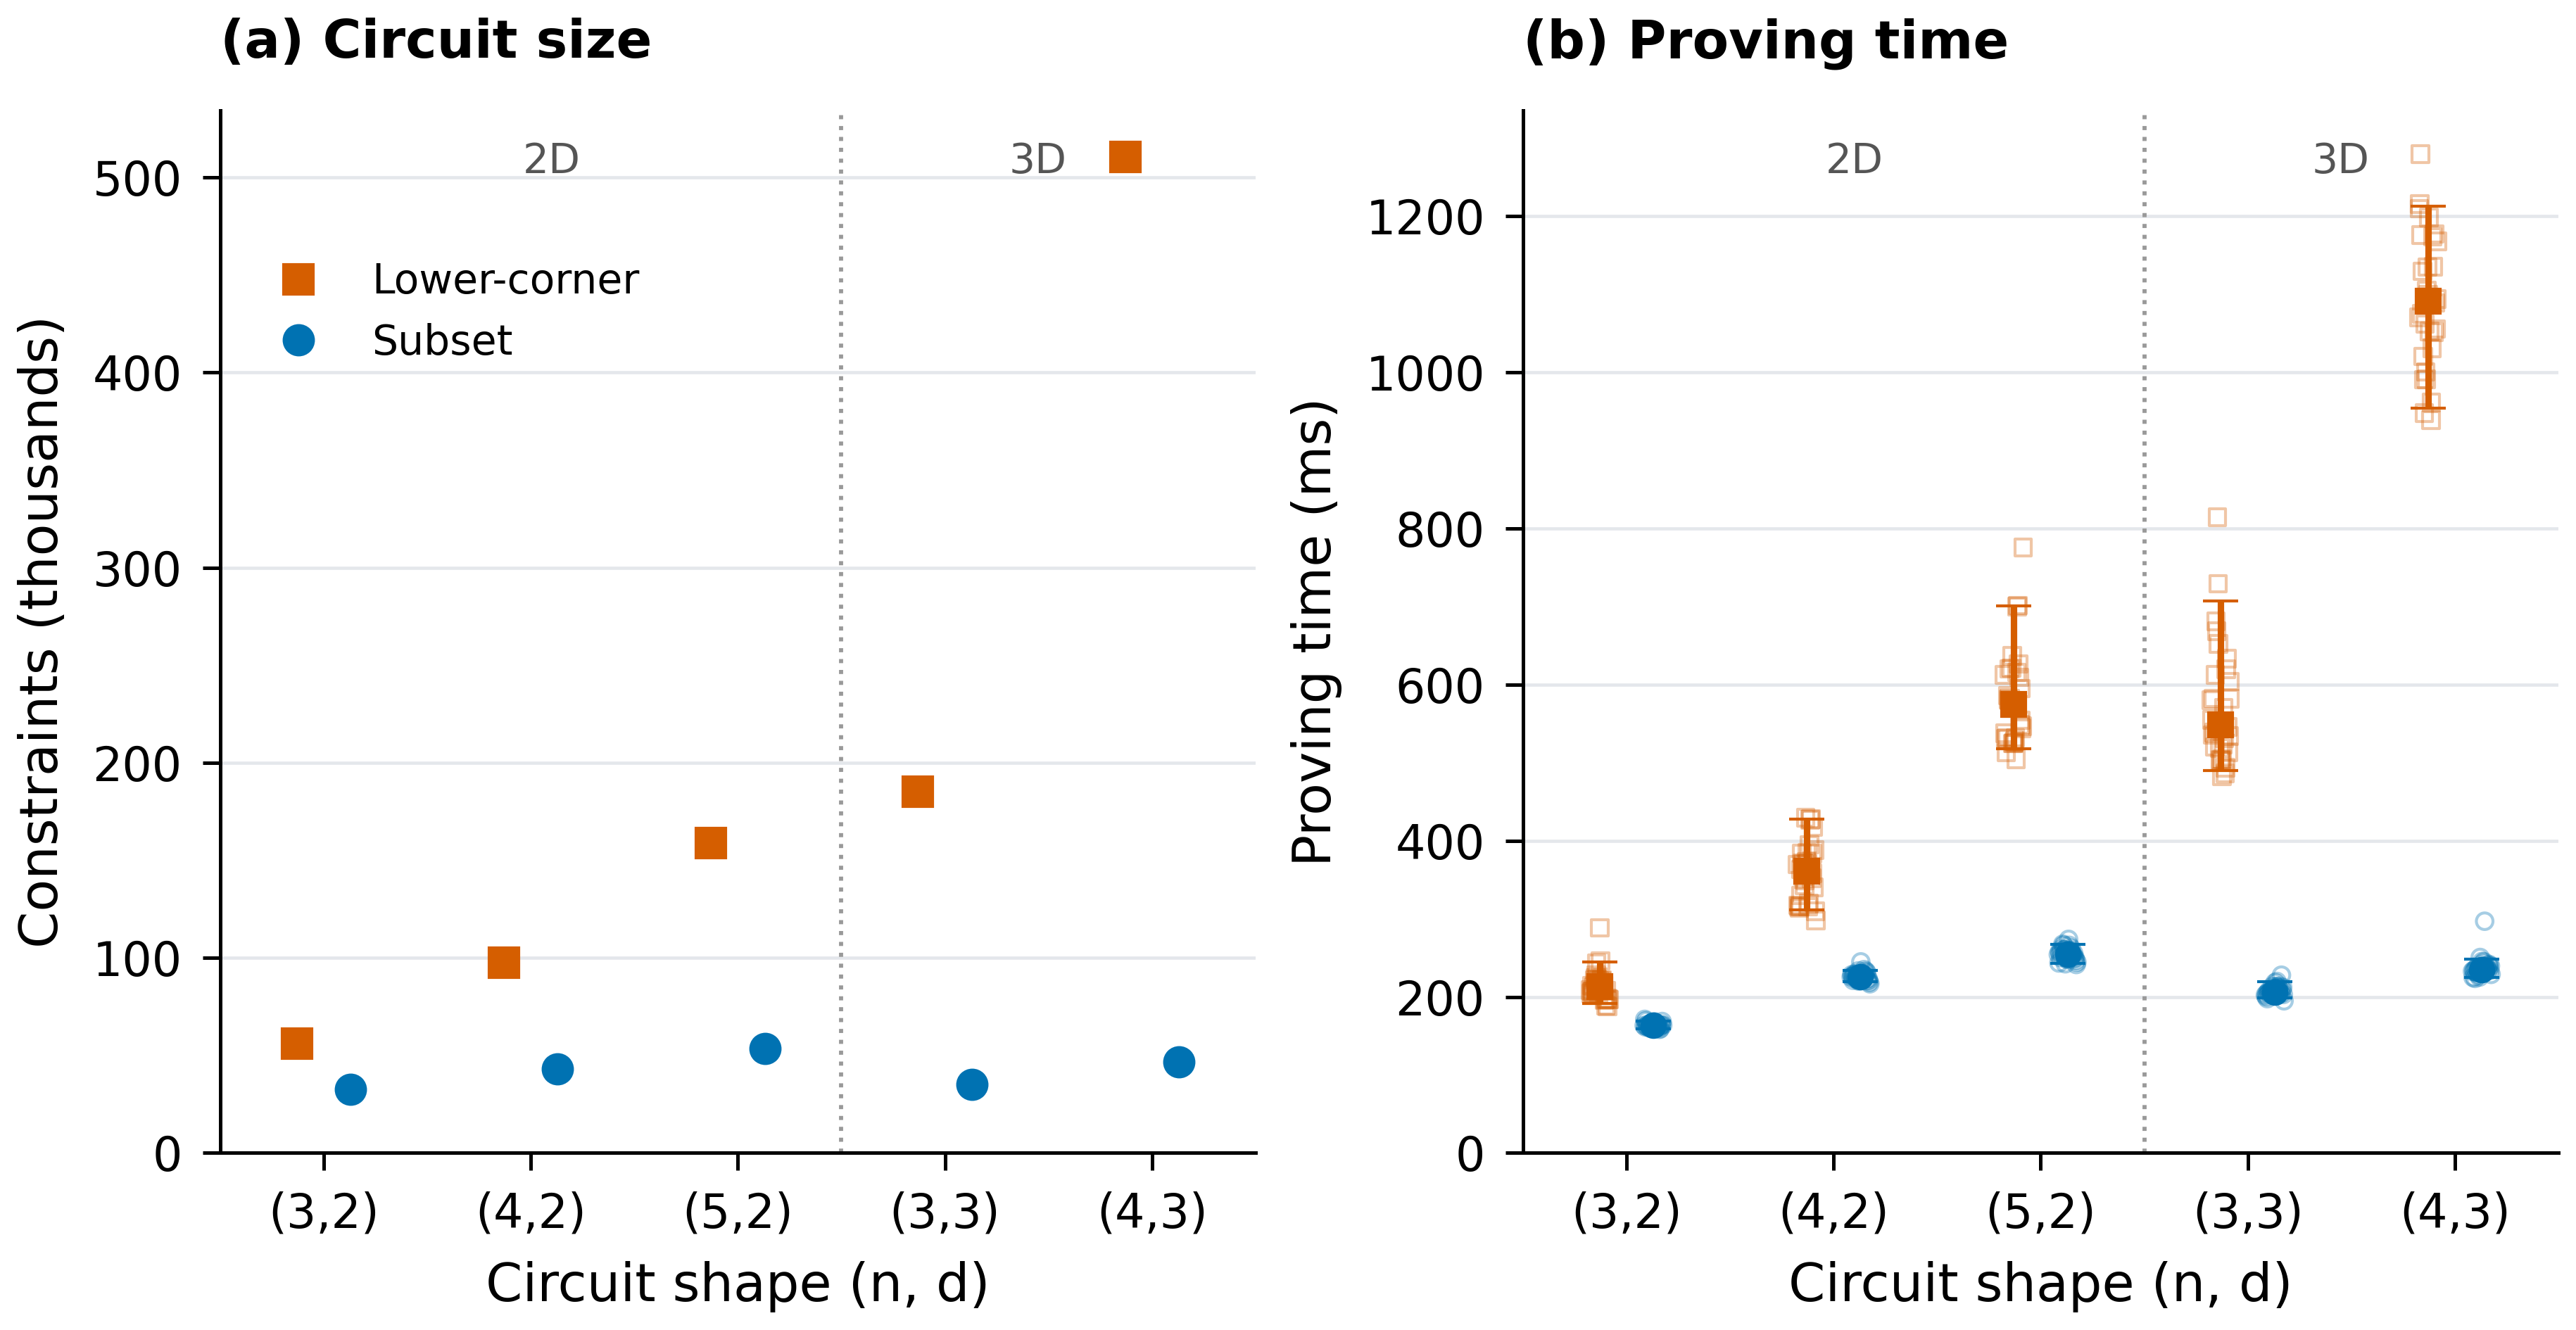
\includegraphics[width=\linewidth]{backend_costs.png}
\caption{R1CS size and proving time for the two backends on the Apple M1 platform. Small points in the timing panel show all 30 observations per circuit shape and backend (300 total); large markers are medians and intervals span the empirical p5--p95 range, not confidence intervals. Backend batches were not interleaved.}\label{fig:scaling}
\end{figure}

Subset enumeration has fewer constraints in every tested configuration with $k=n-1$. For example, at $(n,d)=(4,3)$, lower-corner reachability requires 510,362 constraints and has a median proving time of 1090.95 ms; the subset backend requires 46,737 constraints and 234.93 ms. The observed ratio of approximately 4.64 is descriptive for the specified test platform, because the backend batches were not interleaved. It is not a universal speedup corrected for environmental variation, and smaller circuits do not by themselves establish the same advantage at every size.

\subsubsection{Resource-limited compilation scalability}
Figure~\ref{fig:compilegrowth} and Table~\ref{tab:compilegrowth} summarize 32 resource-bounded compilation invocations. Of these, 27 completed; five were terminated after the sampled RSS reached the 3 GiB threshold, indicated by \texttt{RL}. At $(d,n)=(2,16)$, lower-corner reachability has 3,509,645 constraints, compared with 181,194 and 308,978 constraints for subsets with omissions $b=n-k$ equal to one and two. At $(d,n,k)=(3,12,6)$, the balanced-threshold subset circuit already has 962,018 constraints. We do not assign estimated counts to unfinished builds or claim that they are theoretically uncomputable.

\begin{table}[htbp]\centering\small
\caption{Resource-limited R1CS compilation sweep with complete signature and geometric constraints. \texttt{RL} indicates termination before a count was obtained.}\label{tab:compilegrowth}
\begin{tabular}{rrrrrr}\toprule
$d$&$n$&Lower corner&Subset $b=1$&Subset $b=2$&Subset $k=n/2$\\\midrule
2&4&97,493&42,918&43,160&43,160\\
2&8&509,277&86,354&97,734&111,776\\
2&12&1,544,390&132,447&181,221&675,759\\
2&16&3,509,645&181,194&308,978&RL\\
3&4&510,362&46,737&47,099&47,099\\
3&8&RL&95,153&112,213&133,255\\
3&12&RL&147,506&220,640&962,018\\
3&16&RL&203,793&395,417&RL\\\bottomrule
\end{tabular}\end{table}

\begin{figure}[htbp]\centering
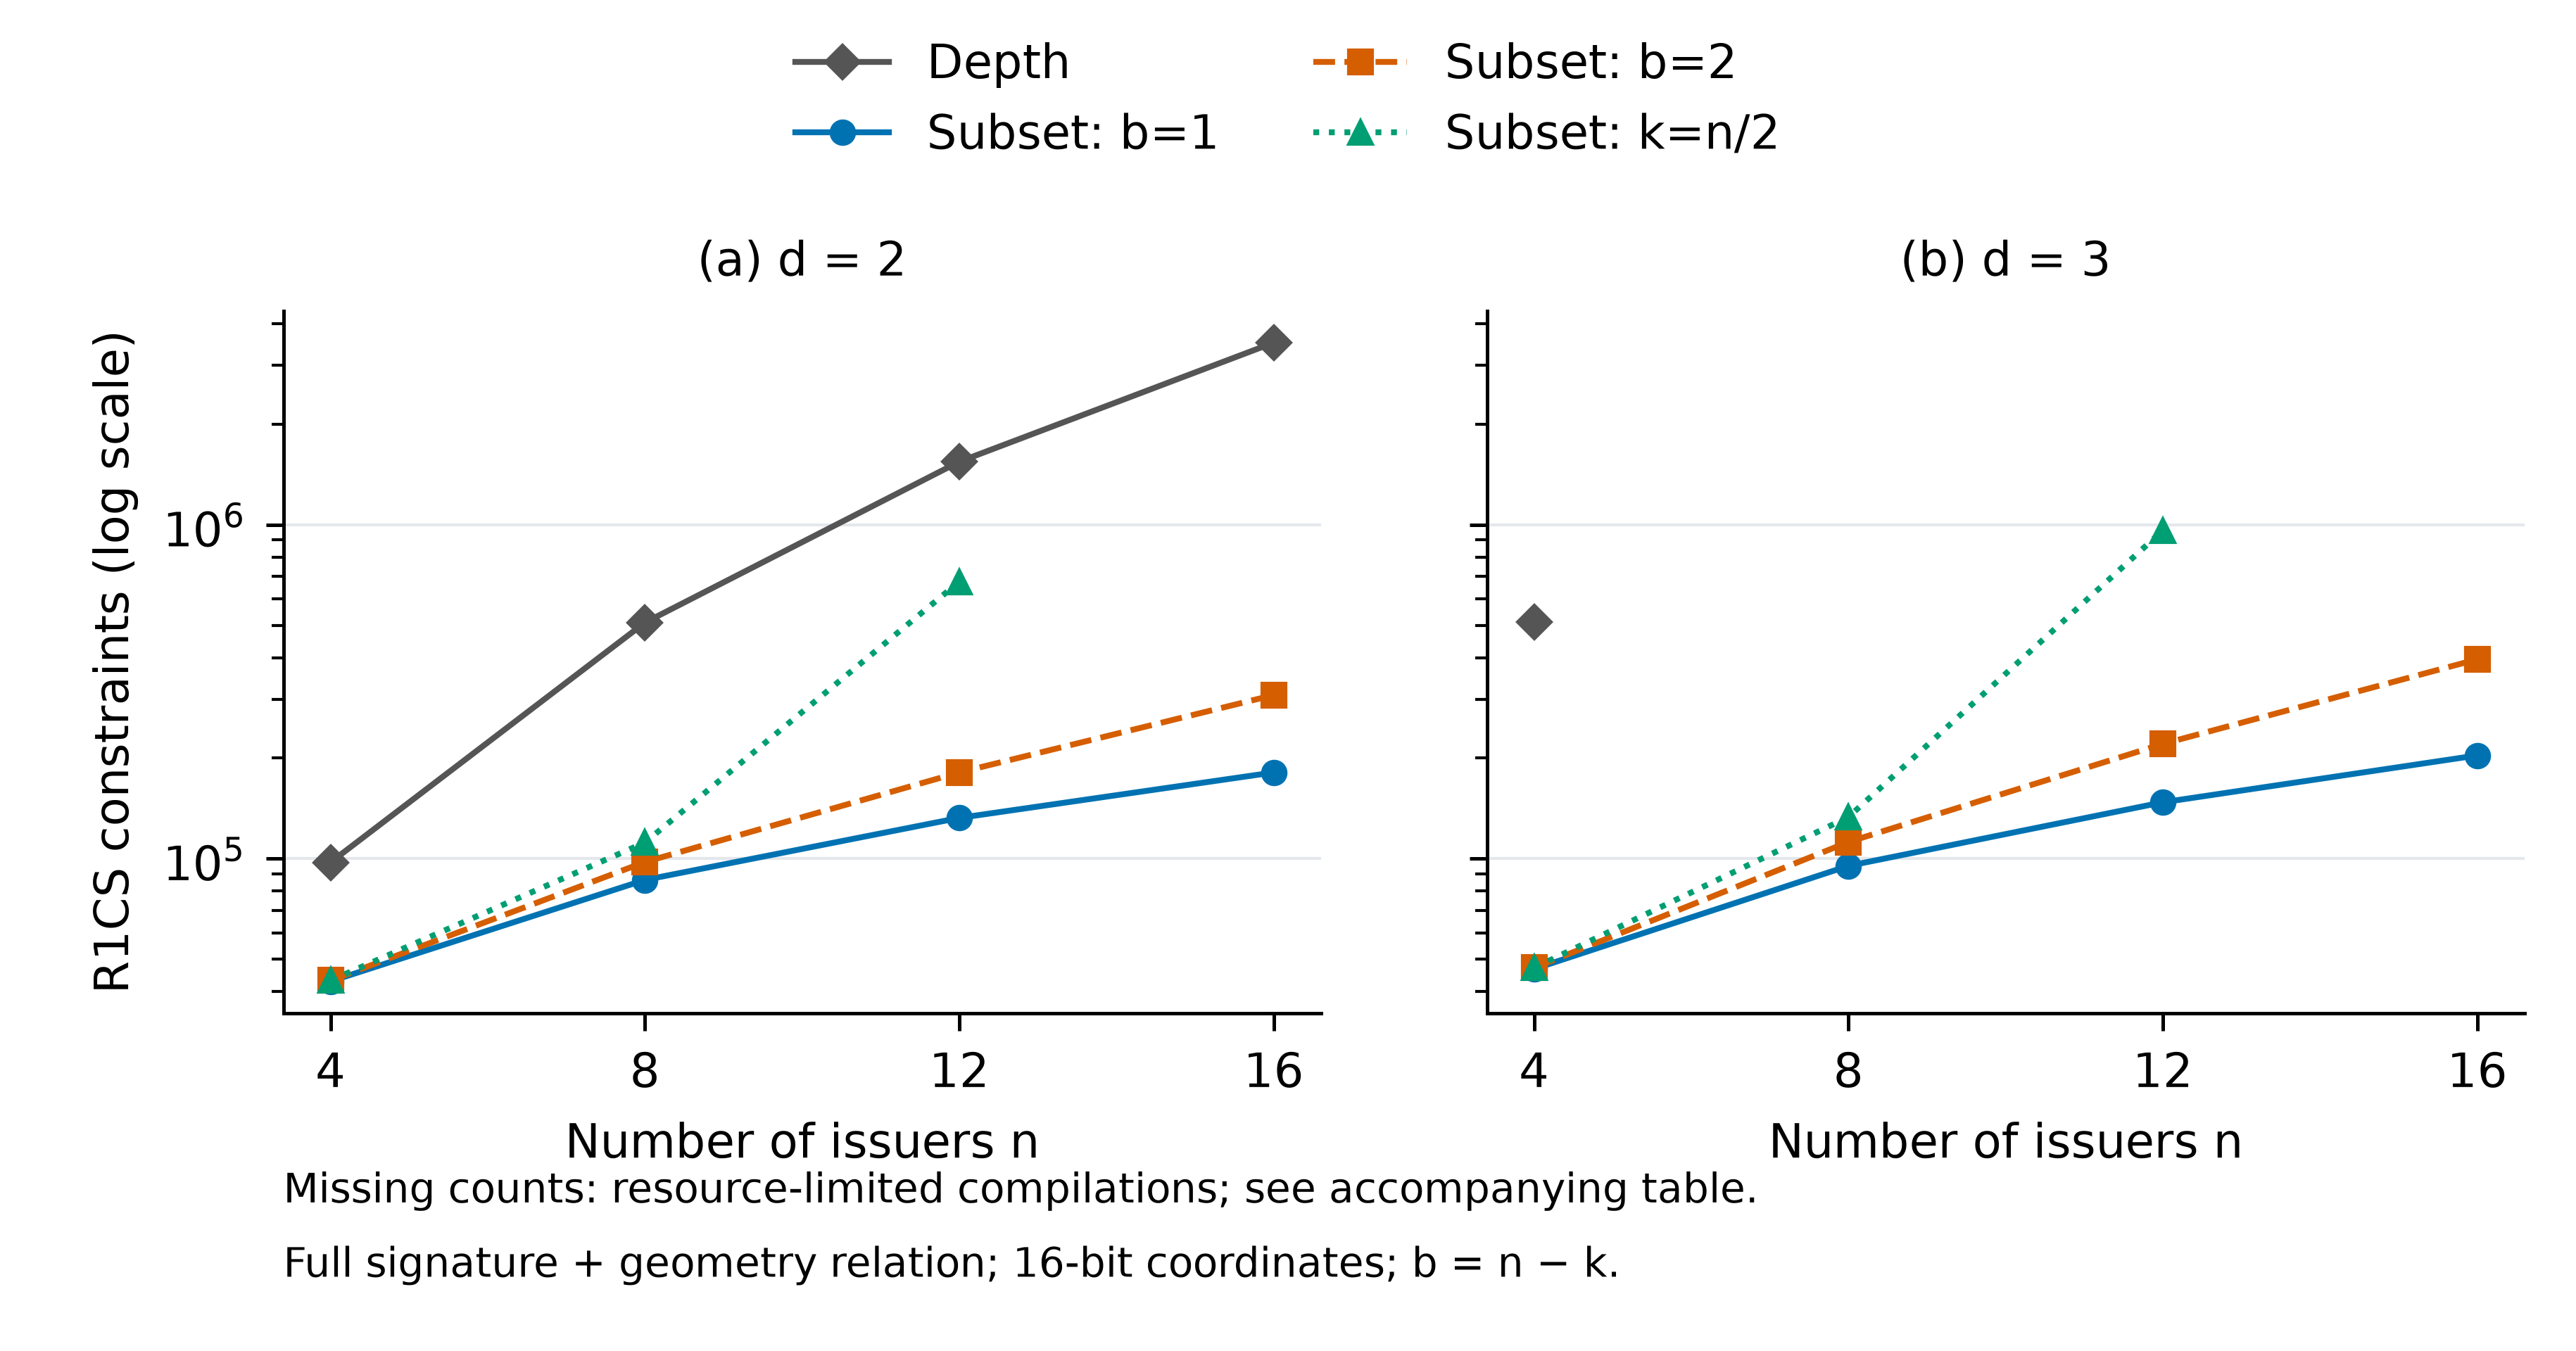
\includegraphics[width=\linewidth]{compile_scalability.png}
\caption{Resource-limited sweep of full R1CS constraint counts. Missing markers correspond to terminated compilations, not zero constraints; connecting lines are visual guides. These are compilation results, not large-circuit proving times.}\label{fig:compilegrowth}
\end{figure}

Taken together, the direct measurements and compilation results favor subset enumeration for the tested small omission budgets $b=f+r$. As $k$ approaches half the source count, however, the number of subsets $\binom nk$ grows rapidly and can diminish the advantage. The evidence supports backend selection for particular tested scales and thresholds, rather than a universal optimum across dimensions, source populations, and hardware.

\section{Discussion and system limitations}
While our evaluation demonstrates the soundness and efficiency of zero-knowledge spacetime compliance over finite domains, several system-level considerations govern its deployment in vehicular networks:
\begin{enumerate}
\item \textbf{Physical calibration and common-mode bias.} Cryptographic proofs guarantee computation integrity over authenticated intervals but cannot verify whether those intervals physically enclose the true event $z^*$. As illustrated by the retrospective single-receiver GNSS diagnostic in Appendix A, a static uncertainty envelope calibrated on an initial time segment (covering 76/78 epochs) covered only 2/69 epochs in a subsequent segment due to temporal drift. Practical deployments therefore require online sensor calibration, conservative quantization envelopes, and cross-provider diversity to mitigate correlated multipath or clock biases.


\item \textbf{Roster availability and gateway state management.} Requiring signatures from a fixed roster of $n$ issuers prevents provers from selectively dropping unfavorable observations, but allows a single unreachable or non-responsive issuer to cause a protocol abort. Extending the circuit with Merkle-tree roster commitments to support dynamic $n$-of-$N$ active issuer subsets, alongside distributed nonce persistence, rate limiting, and report deduplication across replicated gateways, is a natural direction for production V2X infrastructures.


\item \textbf{Privacy scope and hardware profiling.} Zero-knowledge proofs conceal the signed spacetime intervals from the gateway, but do not encrypt the report payload $R$ or prevent location inference under unrestricted adaptive policy queries. Finally, our benchmarks measure Groth16 proving latencies on an Apple M1 workstation; deploying the prover on resource-constrained automotive on-board units (OBUs) will require profiling energy consumption, V2I communication latency, and multi-party trusted setup ceremonies (or transparent SNARK backends).
\end{enumerate}


\subsection{Parameter choices and V2X interoperability}
The implemented Groth16 proving stack uses the BN254 pairing-friendly curve because the chosen gnark library supports its R1CS setup, proofs, and efficient in-circuit twisted-Edwards EdDSA/MiMC signature checks. BN254 offers approximately 100-bit security under contemporary pairing-field discrete-logarithm estimates, below a modern 128-bit long-term deployment target; these measurements therefore characterize a prototype configuration, not a 128-bit security claim. A production migration could use an appropriately selected higher-security pairing curve and remeasure setup, prover, verifier, and circuit costs. The circuit verifies gnark's twisted-Edwards BN254 EdDSA signatures, not Ed25519 or IEEE 1609.2-compliant ECDSA credentials.

In deployed C-ITS infrastructures, certificate-based V2X authenticity typically relies on IEEE 1609.2/ETSI TS 103 097 signatures, including ECDSA over NIST P-256. A practical gateway would first authenticate the V2X certificate chain and bind the authorized credential to a registered issuer identity; the in-circuit evidence signature would require either a separately enrolled SNARK-friendly key or a verified certificate-to-evidence binding. Replacing it with direct P-256 verification inside the current BN254 circuit would require non-native arithmetic and an independent cost and security evaluation. The MiMC primitive follows the pinned gnark-crypto v0.19.0 BN254/fr implementation, which uses 110 MiMC rounds, exponent five, and round constants derived from the literal seed ``seed'' through legacy Keccak-256; these parameters were not customized in this study. No compatibility, certificate-conversion, or 128-bit end-to-end performance claims are made for the evaluated prototype.

\section{Conclusion}
We have presented a zero-knowledge spacetime compliance certification framework for vehicular crowdsensing under measurement uncertainty and Byzantine evidence. Rather than certifying a single concealed coordinate, our method constructs the robust feasible set of states supported by at least $k = n - f - r$ signed uncertainty intervals and evaluates a four-valued compliance rule (Valid, Invalid, Ambiguous, and Inconsistent), accepting reports only when the feasible set is nonempty and wholly contained within the authorized policy.

We realized this relation in two exact Groth16/BN254 circuit backends---lower-corner reachability and threshold-subset enumeration---paired with a challenge-bound verification gateway. Across 12 calibrated synthetic conditions satisfying the fault and coverage budgets, the robust rule exhibited no wrong decisive classifications in the evaluated within-budget cases while improving mean decisive coverage to 87.52\% over a fixed-margin baseline (75.63\%). For small omission budgets, the subset backend achieves 164-byte proofs and 163--255 ms median proving times on an Apple M1. Future work will investigate online uncertainty calibration across heterogeneous vehicular sensors, dynamic threshold roster commitments, and end-to-end evaluation on embedded automotive hardware.

\section*{Data and code availability}
The proof prototype, synthetic evaluations, benchmark logs, and reproducibility records are hosted in the separate code and experiments repository at \url{https://github.com/js110/ZCRSC-PAPER}. Generated evaluation data can be reproduced using the provided scripts. The third-party UrbanNav and GraphGNSSLib data are not redistributed by the authors and should be obtained from the original providers.
\section*{Funding}
This study received partial support from the Heilongjiang Provincial University Teacher Scientific Research Business Fee (2018-KYYWF0941), the Heilongjiang Provincial Natural Science Foundation Joint Fund Cultivation Project (PL2024F002), the National Foreign Expert Key Support Project (D2O25O185), and the Heilongjiang Provincial Undergraduate University Excellent Young Teacher Fundamental Research Support Plan (YQJH2024239).
\section*{CRediT authorship contribution statement}
Lili He: Supervision. Sheng Jiang: Methodology, Software, Investigation, Formal analysis. Shuang Chen: Writing -- original draft. Lei Zhang: Supervision, Corresponding author.

\appendix
\section{Retrospective single-receiver calibration diagnostic}\label{app:receiver}
To examine whether a fixed uncertainty envelope transfers across different time periods, we perform an exploratory diagnostic on the TST2 reference data from GraphGNSSLib~\citep{GraphGNSSData}. The sequence contains 157 matched reference epochs associated with precomputed RTKLIB 2.4.2 kinematic combined solutions. Horizontal east and north residuals are calculated relative to the reference coordinates supplied with the repository, without fitted alignment, bias correction, filtering, or interpolation. Vertical errors are excluded because the elevation datum and antenna-related conventions have not been established.

The first 78 epochs in chronological order are reserved for calibration, the next ten form a gap, and the final 69 are used for evaluation. If $e_j$ and $n_j$ are the east and north residuals at epoch $j$, define
\[
s_j=\max\bigl(|e_j|,|n_j|\bigr).
\]
The 76th ordered score among calibration epochs gives a square axis-aligned envelope with half-width 0.863506 m. We also test the east/north $3\sigma$ rectangular envelope reported by the original solution file. Table~\ref{tab:receiver} counts the epochs for which each envelope contains the reference position.

\begin{table}[htbp]\centering\small
\caption{Reference-position containment in the single-receiver diagnostic (contained epochs / available epochs). Temporal epochs are not independent trials.}\label{tab:receiver}
\begin{tabularx}{\linewidth}{@{}Xrr@{}}\toprule
Envelope rule&Calibration (78)&Evaluation (69)\\\midrule
Solution-reported $3\sigma$ rectangle&8/78&0/69\\
Empirically calibrated square (0.863506 m half-width)&76/78&2/69\\\bottomrule
\end{tabularx}
\end{table}

The empirical square contains 76 of 78 reference positions in calibration but only 2 of 69 in the subsequent evaluation segment. For the reported $3\sigma$ rectangle, the corresponding counts are 8/78 and 0/69. The median horizontal residual increases from 0.869 m to 1.038 m, and the maximum evaluation residual reaches 1.522 m. Under this particular sequence and rule, the uncertainty bound estimated from earlier data fails to cover most of the later observations.

Because the series exhibits temporal dependence and the solution is based on forward/backward combined processing, the 157 epochs cannot be treated as independent, identically distributed trials. Nor can the retrospective split establish an online calibration guarantee. The diagnostic uses neither real multisource signed evidence nor the complete vehicular verification protocol; it serves only to illustrate why the physical coverage premise of Section~4 requires independent empirical validation. Figure~\ref{fig:receiver} shows the residual sequence and the fixed threshold.

\begin{figure}[htbp]\centering
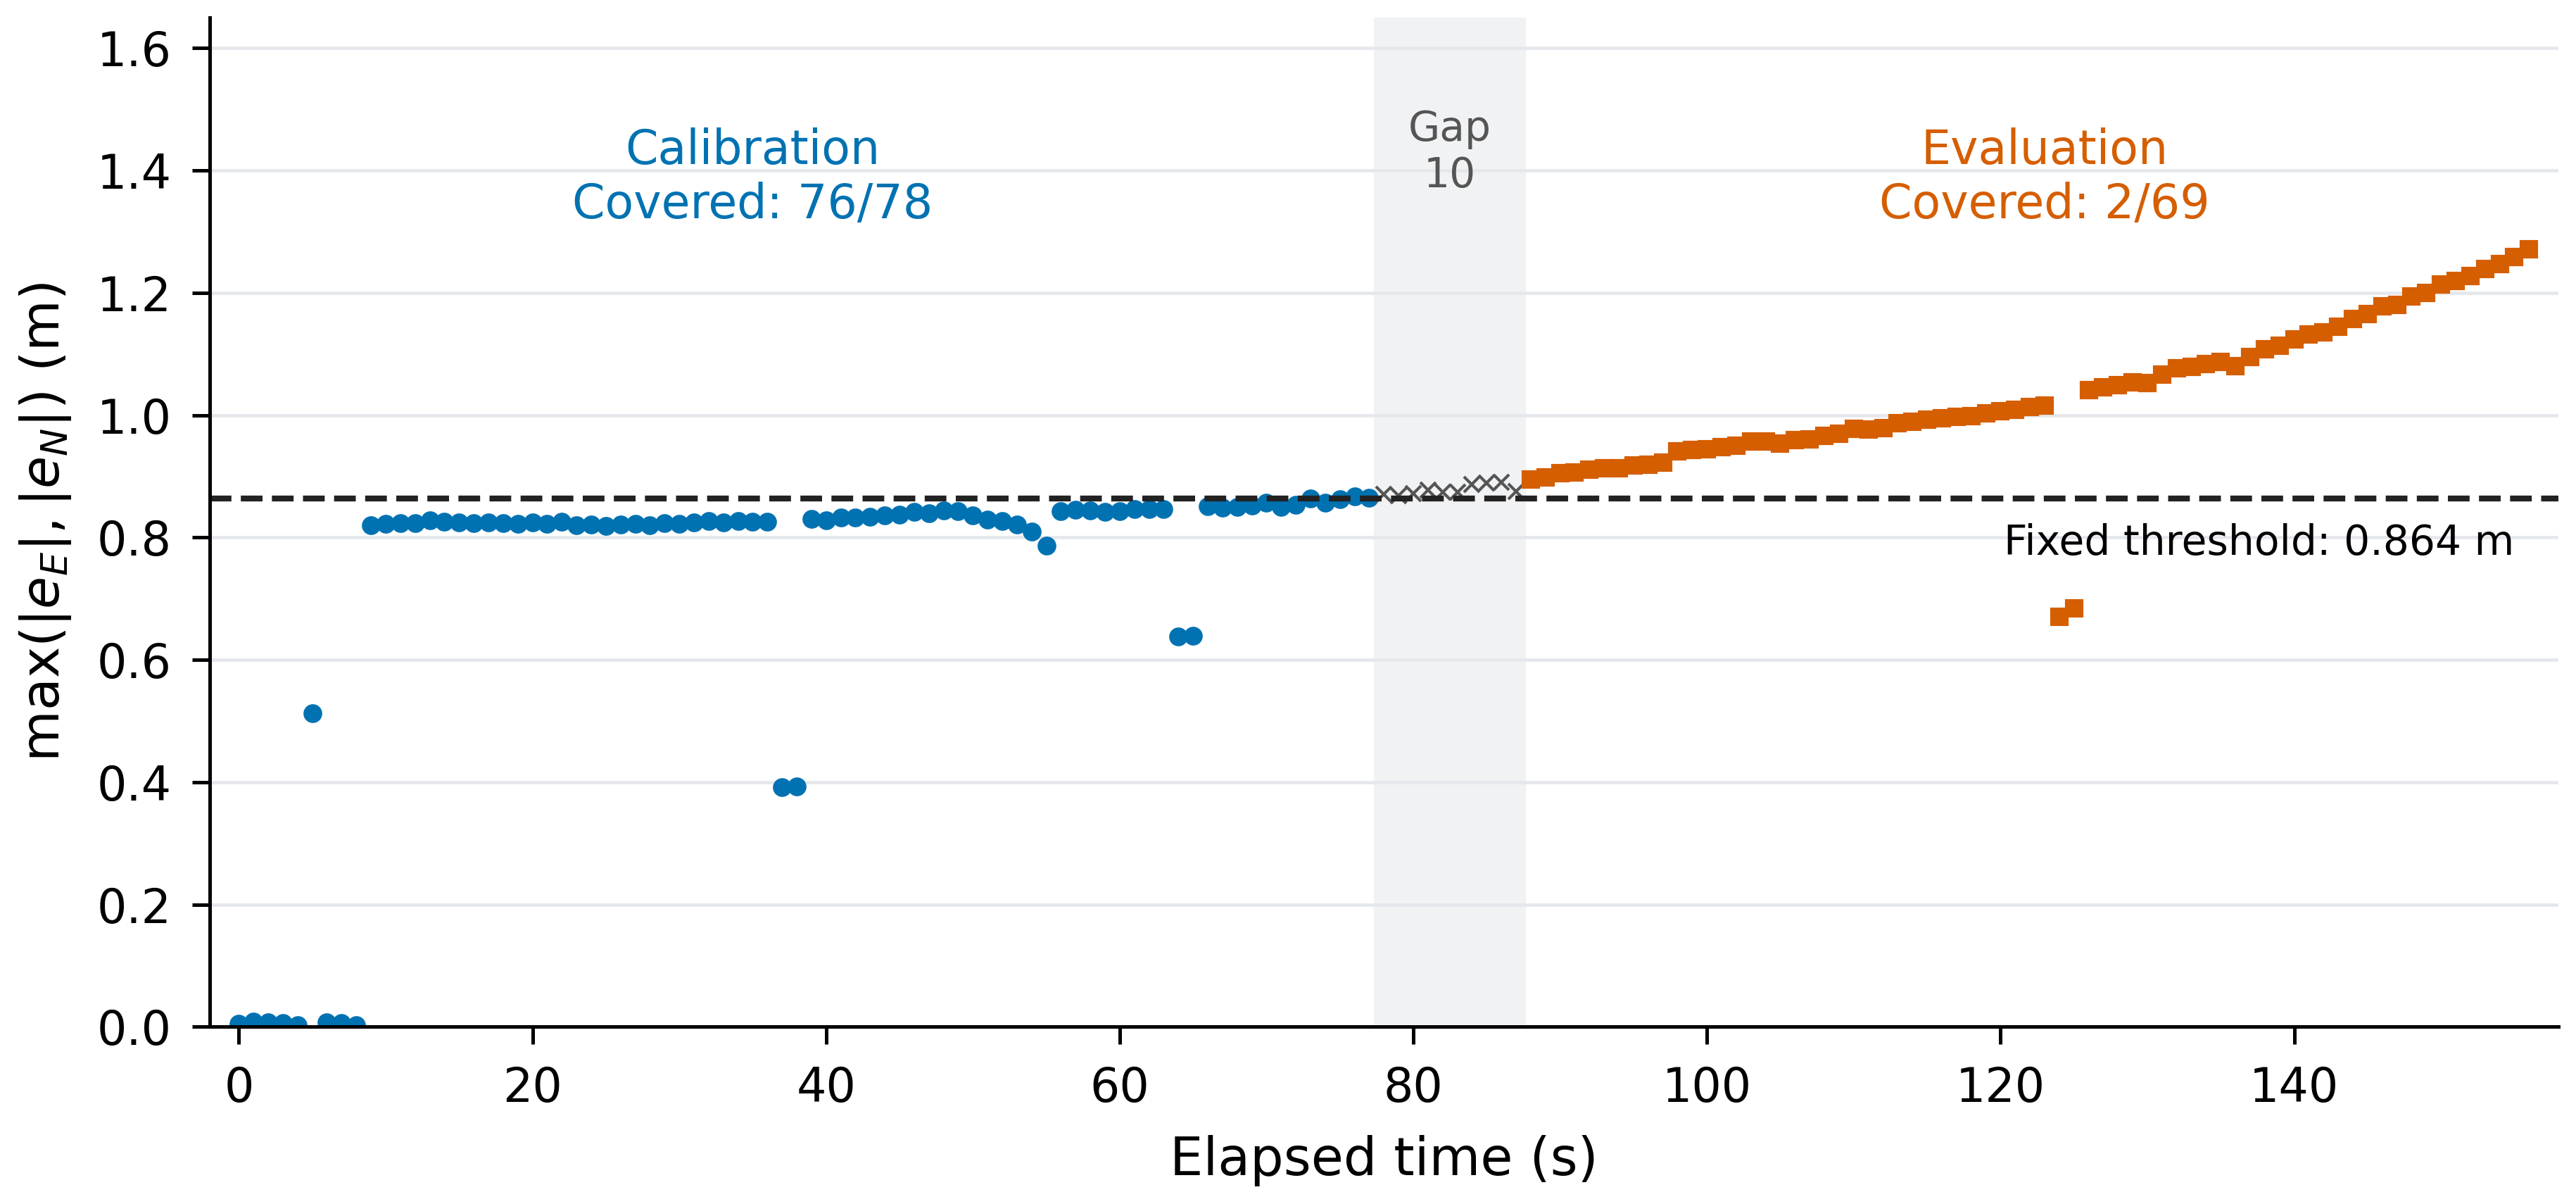
\includegraphics[width=\linewidth]{receiver_diagnostic.png}
\caption{Horizontal residual diagnostic for one stationary receiver. All 157 matched epochs are plotted, with a dashed line showing the 0.863506 m square half-width obtained from the calibration segment. Serial dependence and combined processing prevent interpreting this as online coverage performance.}\label{fig:receiver}
\end{figure}

\bibliographystyle{elsarticle-harv}
\bibliography{references}
\end{document}
